\documentclass[a4paper,10pt,oneside]{book}

%% Packages order is important
\usepackage[utf8]{inputenc}
\usepackage[T1]{fontenc}
%\usepackage[left=3.175cm, marginparwidth=2.825cm, marginparsep=3mm]{geometry}
%\usepackage{marginnote}
%\reversemarginpar
\usepackage{lastpage}

\usepackage[hidelinks]{hyperref}
\usepackage{amsmath}
\usepackage{amssymb}
\usepackage{bbm}
\usepackage{amsthm}
\usepackage{mathtools}
\usepackage{tikz}
\usepackage{braids}
\usepackage{xifthen}
\usepackage{datetime}
\usepackage{graphicx}
\usepackage{cleveref}


\setlength{\marginparwidth}{3.5cm}

\usepackage{showkeys}
% Enable showkeys for \cref and \Cref
% tex.stackexchange.com/questions/139698/usiong-showkes-and-cleveref-together
\makeatletter
  \SK@def\cref#1{\SK@\SK@@ref{#1}\SK@cref{#1}}%
  \SK@def\Cref#1{\SK@\SK@@ref{#1}\SK@Cref{#1}}%
\makeatother
% \renewcommand*\showkeyslabelformat[1]{%
%   \parbox[t]{\marginparwidth}{\raggedright\normalfont\footnotesize\ttfamily#1}}

% \usepackage{showlabels}
% \showlabels{cite}
% \showlabels{eqref}
% \showlabels{cref}
% \showlabels{bibitem}
% \renewcommand*\showlabelsetlabel[1]{%
%   \parbox[t]{\marginparwidth}{\raggedright\normalfont\footnotesize\ttfamily#1}}



%% Theorems

\theoremstyle{plain}
\newtheorem{theorem}{Theorem}[section]
\newtheorem{proposition}[theorem]{Proposition}
\newtheorem{lemma}[theorem]{Lemma}
\newtheorem{corollary}[theorem]{Corollary}

\theoremstyle{definition}
\newtheorem{definition}{Definition}[section]
\newtheorem{example}{Example}[section]

\theoremstyle{remark}
\newtheorem{remark}{Remark}[section]


%% Macros

\newcommand{\N}{\mathbb{N}}
\newcommand{\Z}{\mathbb{Z}}
\newcommand{\Q}{\mathbb{Q}}
\newcommand{\R}{\mathbb{R}}
\newcommand{\M}{\mathcal{M}}
\newcommand{\bm}[1]{\boldsymbol{\mathbf{#1}}}
\DeclarePairedDelimiter\abs{\lvert}{\rvert}
\DeclarePairedDelimiter\norm{\lVert}{\rVert}
\DeclarePairedDelimiter\bra{\langle}{\rvert}
\DeclarePairedDelimiter\ket{\lvert}{\rangle}
\DeclarePairedDelimiterX\braket[2]{\langle}{\rangle}{#1 \delimsize\vert #2}

\DeclareMathOperator{\Fib}{Fib}

\newcommand*\centermathcell[1]{\omit\hfil$\displaystyle#1$\hfil\ignorespaces}
\newcommand{\centermath}[1]{\centerline{\begin{minipage}{\linewidth}#1\end{minipage}}}

% BEGIN FUSION STATE DIAGRAM \fs
\makeatletter
\newcounter{mycounter}
\newcommand{\fs}[3][]{
  \begin{tikzpicture}[scale=0.3,font=\footnotesize,anchor=mid,baseline={([yshift=-.5ex]current bounding box.center)}]
    \def\height{1.5}
    \def\offset{0.5}
    \ifthenelse{\equal{#1}{}}{\def\height{1}}{} % Smaller height if no braiding
    \setcounter{mycounter}{0}
    \@for\el:=#2\do{
      \ifthenelse{\equal{#1}{\value{mycounter}}}{
        \braid at (\value{mycounter},\height) s_1^{-1};
        \stepcounter{mycounter}
      }{
        \stepcounter{mycounter}
        \ifthenelse{\equal{#1}{\value{mycounter}}}{
        }{
          \draw (\value{mycounter}, \height) to (\value{mycounter}, 0);
        }
      }
      \node at (\value{mycounter}, \height+\offset) {$\el$};
    }
    \draw (0, 0) to (\value{mycounter}+1, 0);
    \setcounter{mycounter}{0}
    \@for\el:=#3\do{
      \node at (\value{mycounter}+0.5, -0.6) {$\el$};
      \stepcounter{mycounter}
    }
  \end{tikzpicture}
}
\makeatother

\makeatletter
\newcommand{\fswide}[3][]{
  \begin{tikzpicture}[scale=0.3,font=\footnotesize,anchor=mid,baseline={([yshift=-.5ex]current bounding box.center)}]
    \def\height{1.75}
    \def\offset{0.5}
    \def\widthfactor{2}
    \ifthenelse{\equal{#1}{}}{\def\height{1}}{} % Smaller height if no braiding
    \setcounter{mycounter}{0}
    \@for\el:=#2\do{
      \ifthenelse{\equal{#1}{\value{mycounter}}}{
        \braid[width=\widthfactor cm, height=1.25 cm] at (\widthfactor*\value{mycounter},\height) s_1^{-1};
        \stepcounter{mycounter}
      }{
        \stepcounter{mycounter}
        \ifthenelse{\equal{#1}{\value{mycounter}}}{
        }{
          \draw (\widthfactor*\value{mycounter}, \height) to (\widthfactor*\value{mycounter}, 0);
        }
      }
      \node at (\widthfactor*\value{mycounter}, \height+\offset) {$\el$};
    }
    \draw (0, 0) to (\widthfactor*\value{mycounter}+\widthfactor*1, 0);
    \setcounter{mycounter}{0}
    \@for\el:=#3\do{
      \node at (\widthfactor*\value{mycounter} + \widthfactor*0.5, -0.6) {$\el$};
      \stepcounter{mycounter}
    }
  \end{tikzpicture}
}
\makeatother

\makeatletter
\newcommand{\fswider}[3][]{
  \begin{tikzpicture}[scale=0.3,font=\footnotesize,anchor=mid,baseline={([yshift=-.5ex]current bounding box.center)}]
    \def\height{1.75}
    \def\offset{0.5}
    \def\widthfactor{3}
    \ifthenelse{\equal{#1}{}}{\def\height{1}}{} % Smaller height if no braiding
    \setcounter{mycounter}{0}
    \@for\el:=#2\do{
      \ifthenelse{\equal{#1}{\value{mycounter}}}{
        \braid[width=\widthfactor cm, height=1.25 cm] at (\widthfactor*\value{mycounter},\height) s_1^{-1};
        \stepcounter{mycounter}
      }{
        \stepcounter{mycounter}
        \ifthenelse{\equal{#1}{\value{mycounter}}}{
        }{
          \draw (\widthfactor*\value{mycounter}, \height) to (\widthfactor*\value{mycounter}, 0);
        }
      }
      \node at (\widthfactor*\value{mycounter}, \height+\offset) {$\el$};
    }
    \draw (0, 0) to (\widthfactor*\value{mycounter}+\widthfactor*1, 0);
    \setcounter{mycounter}{0}
    \@for\el:=#3\do{
      \node at (\widthfactor*\value{mycounter} + \widthfactor*0.5, -0.6) {$\el$};
      \stepcounter{mycounter}
    }
  \end{tikzpicture}
}
\makeatother

\newcommand{\fsfused}[5]{
  \begin{tikzpicture}[scale=0.3,font=\footnotesize,anchor=mid,baseline={([yshift=-.5ex]current bounding box.center)}]
    \def\height{1.75}
    \def\offset{0.5}
    \node at (1, \height+\offset) {$#2$};
    \node at (2, \height+\offset) {$#3$};
    \draw (0.5, 0) to (2.5, 0);
    \draw (1, \height) to [bend left=-30] (1.5, 1);
    \draw (2, \height) to [bend left=30] (1.5, 1);
    \draw (1.5, 1) to (1.5, 0);
    \node at (0.75, -0.6) {$#1$};
    \node at (2.25, -0.6) {$#4$};
    \node at (2, 0.7) {$#5$};
  \end{tikzpicture}
}

\newcommand{\fsfuseddouble}[9]{
  \begin{tikzpicture}[scale=0.3,font=\footnotesize,anchor=mid,baseline={([yshift=-.5ex]current bounding box.center)}]
    \def\height{1.75}
    \def\offset{0.5}
    \node at (1, \height+\offset) {$#2$};
    \node at (2, \height+\offset) {$#3$};
    \node at (3, \height+\offset) {$#6$};
    \node at (4, \height+\offset) {$#7$};
    \draw (0.5, 0) to (4.5, 0);
    \draw (1, \height) to [bend left=-30] (1.5, 1);
    \draw (2, \height) to [bend left=30]  (1.5, 1);
    \draw (3, \height) to [bend left=-30] (3.5, 1);
    \draw (4, \height) to [bend left=30]  (3.5, 1);
    \draw (1.5, 1) to (1.5, 0);
    \draw (3.5, 1) to (3.5, 0);
    \node at (2,     0.5) {$#4$};
    \node at (0.75, -0.6) {$#1$};
    \node at (2.5,    -0.6) {$#5$};
    \node at (4,     0.5) {$#8$};
    \node at (4.25, -0.6) {$#9$};
  \end{tikzpicture}
}

\newcommand{\fsfusedbraided}[5]{
  \begin{tikzpicture}[scale=0.3,font=\footnotesize,anchor=mid,baseline={([yshift=-.5ex]current bounding box.center)}]
    \def\height{3}
    \def\offset{0.5}
    \node at (1, \height+\offset) {$#2$};
    \node at (2, \height+\offset) {$#3$};
    \braid at (1, \height) s_1^{-1};
    \draw (0.5, 0) to (2.5, 0);
    \draw (1, 1.5) to [bend left=-30] (1.5, 1);
    \draw (2, 1.5) to [bend left=30] (1.5, 1);
    \draw (1.5, 1) to (1.5, 0);
    \node at (0.5, -0.6) {$#1$};
    \node at (2.5, -0.6) {$#4$};
    \node at (2, 0.7) {$#5$};
  \end{tikzpicture}
}

% END FUSION STATE DIAGRAM


\begin{document}

\title{Non-Abelian Anyons:\\Topological Quantum Computation and\\Exclusion Principles}
% \title{Topological Quantum Computation and Exclusion Principles for Non-Abelian Anyons}
\author{Viktor Qvarfordt}
\newdateformat{isodate}{\THEYEAR-\twodigit{\THEMONTH}-\twodigit{\THEDAY}}
\date{\isodate\today\ \currenttime}
\maketitle
\tableofcontents
\newpage




%%%%%%%%%%%%%%%%%%%%%%%%%%%%%%%%%%%%%%%%%%%%%%%%%%%%%%%%%%%%%%%%%%%%%%%%%%%%%%%%




Layout

\begin{enumerate}
  \item Aharonov-Bohm effect
  \item Statistics in two (and three) dimensions
  \item Lieb-Thirring inequalities and lower bound for the kinetic energy
  \item Quantum computation
  \begin{enumerate}
    \item Topological quantum computation
    \item Fibonacci anyons
    \item Braiding matrices
  \end{enumerate}
\end{enumerate}

\chapter{Introduction}

{ % Parsa intro knots
Non-trivial knots exist only in three dimensions. If the number of dimensions are fewer it is impossible to form a knot on a strand

``Any fewer dimensions, and it is impossible to form a knot in a strand, since there is no “under” or “over,” just “next to.” Any more dimensions and there is too much spatial freedom, which will make knots unravel, since one can always move one strand past another by pushing it into one of the extra dimensions, where it may pass unhindered.''
}

\vspace{0.5cm}
\hrule
\vspace{0.5cm}

{ % Parsa intro config space
Consider $n$ identical quantum mechanical particles on a spatial manifold $M$.
% If the particles are allowed to occupy the same point in space the exchange statistics is trivial, such particles are called Bosons.
The corresponding configuration space is defined as
\begin{align*}
  \mathcal{C}_n = \frac{M^n - \Delta_n}{S_n}.
\end{align*}
By removing the set
\begin{align*}
  \Delta_n = \{(x_1,\ldots,x_n) \in M^n \mid x_i = x_j \text{ for some } i, j\}
\end{align*}
of configurations where particles occupy the same point in space (known as a ``hard-core'' condition) we allow for non-trivial exchange statistics (as we shall shortly see). Without this condition we get bosons. To model the fact that the particles are identical, we form the quotient of $M^n - \Delta_n$ by the symmetric group $S_n$, in this way all permutations of the $n$ particles are considered to be the same configuration.

\vspace{0.5cm}
\hrule
\vspace{0.5cm}

\textbf{Motivering för att studera fundamentalgruppen} The state of a quantum system is described by a wave function $\psi$ defined as a section of the vector bundle with fiber $h$ over the configuration space $\mathcal{C}$, where $h$ is a Hilbert space over $\mathbb{C}$. We take $h$ to be finite dimensional, i.e. $h = \mathbb{C}^k$, where $k$ can be seen as the number internal degrees of freedom of the quantum system.
% Example of infinite dimensional is the landau states; free electron in constant magnetic field.
Locally, the wave function is a function $\mathcal{C} \to \mathbb{C}^k$.

Evolution of a quantum system is described by unitary transformations.

\vspace{0.5cm}
\hrule
\vspace{0.5cm}


Consider an exchange of particles, that is, take $n$ identical particles on $M$ with given positions and move them around until they are back at some permutation of the original positions. Such an exchange is described by a loop in the configuration space $\mathcal{C}^n$. More precisely, a loop $\alpha(t)$ in $\mathcal{C}^n\times[0,1]$, where $t \in [0,1]$ is considered as the time parameter, corresponds to world-lines of particle trajectories in $M\times[0,1]$. The corresponding world-lines are constructed by choosing a representative of $\alpha(t)$ in $M^n\times[0,1]$ and then projecting the coordinates of each particle into $M\times[0,1]$.

In this way, each loop in $\mathcal{C}^n$ corresponds a classical motion of the particles along world-lines starting and ending in the same configuration. The corresponding quantum mechanical dynamics is obtained by quantizing the system via the path integral formulation \cite{feynmann path integral,nakahara}. In this model, the contributions can be split into homotopically inequivalent ... \cite{feynmann path integrals indistinguishable particles}

\hrule

... Proofs of these results can be found in \cite{oskar} and \cite{configuration spaces}


\subsection{Example: Exchange of two identical particles in a flat geometry}

The configuration space of $n = 2$ identical particles (with hard-core condition) in $\mathbb{R}^m$ is given by
\begin{align*}
  \mathcal{C} = \frac{(\R^m)^2 - \Delta}{S_2}.
\end{align*}
The space $(\R^m)^2$ can be factored as $\R^m_\text{cm} \times \R^m_\text{rel}$ where $\R^m_\text{cm}$ gives the coordinates of the center of mass for the two particles and $\R^m_\text{rel}$ gives the relative coordinate of the two particles. Let $x_1, x_2 \in \R^m$ be the (absolute) coordinates of the two particles, so that $x = (x_1, x_2) \in \mathcal{C}$. We then define
\begin{align*}
  x_\text{cm} = \frac{1}{2}(x_1 + x_2), \quad
  x_\text{rel} = \frac{1}{2}(x_1 - x_2).
\end{align*}
Now, $\Delta = \{(x_1, x_2) \in (\R^m)^2 \mid x_1 = x_2\}$ is precisely the origin of $\R^m_\text{rel}$.
Furthermore, quotiening with $S_2$ corresponds to quotiening with the equivalence relation $x_\text{rel} \sim x_\text{rel}' \iff x_\text{rel} = - x_\text{rel}'$. Thus we have
\begin{align*}
  \mathcal{C} = \R^m_\text{cm} \times \underbrace{(\R^m_\text{rel} - \{0\}) / \sim}_{\mathcal{C}_\text{rel}}
\end{align*}
where we see that the center of mass enters as a gauge freedom, it contributes trivially to the topology of the configuration space.

The real projective $m$-space is defined as
\begin{align*}
  \R\mathbb{P}^m = (\R^{m+1}-\{0\})/\sim_\text{proj}, \quad x \sim_\text{proj} y \iff \exists \lambda \ne 0 : x = \lambda y,
\end{align*}
thus we have
\begin{align*}
  \mathcal{C}_\text{rel} \cong \R_+ \times \R\mathbb{P}^{m-1}.
\end{align*}
Since the fundamental group has the property that $\pi_1(X\times Y) \cong \pi_1(X) \times \pi_1(Y)$ for path connected spaces $X$ and $Y$ we have
\begin{align*}
  \pi_1(\mathcal{C}) = \pi_1(\R\mathbb{P}^{m-1}) =
  \begin{cases}
    \Z & m = 2 \\
    \Z_2 & m \ge 3
  \end{cases}
\end{align*}

In two dimensions $m=2$, the space $\mathcal{C}_\text{rel}$ can be though of as the half plane $\R^2_{y \ge 0} - \{ 0 \}$ with $x$ and $-x$ identified, or geometrically as a punctured cone.




\vspace{0.5cm}
\hrule
\vspace{0.5cm}

\textbf{Higher dimensional representations of $S_n$}

Higher-dimensional realizations of $S_n$ give rise to particles called plektons. \cite{fröhlich} avsnitt 1.6 och mer ingående i avsnitt 3.


\vspace{0.5cm}
\hrule
\vspace{0.5cm}



TODO: Describe with $\ket{\psi_1}\ket{\psi_2} = e^{i\theta} \ket{\psi_2}\ket{\psi_1}$


...to study properties of anyons, more specifically non-abelian anyons. We shall presently describe precisely what exactly an anyon is.

..the focus is twofold; anyons localized and trapped in a potential allowing us to move the anyons in a controlled manner. and consider how quantum computation and quantum memory can be realized in the topological properties of anyons. Free anyons give rise to an exclusion principle, similar to that of fermions.

Let us now define exactly what is meant by an anyon. We begin with the simplest case, abelian anyons

\section{The braid group}

The braid group $B_n$ (representing braids on $n$ strands) is the group with generators $\sigma_1, \ldots, \sigma_{n-1}$ and relations
\begin{equation}\label{braid relations}
  \begin{aligned}
    \sigma_i \sigma_j &= \sigma_j \sigma_i \quad\text{if}\quad |i-j| \ge 2, \\
    \sigma_i \sigma_{i+1} \sigma_i &= \sigma_{i+1} \sigma_i \sigma_{i+1}.
  \end{aligned}
\end{equation}

\section{Gague invariance of the anyonic phase}

All that can be observed is the difference in phase when two particles have been winded around each other. How the phase is affected before the particles meet is non-physical, we are free to choose this so long as the choice respects the result of a complete winding of particles; this is a gauge invarianve.


\section{The Aharonov-Bohm effect}

Electron beam split around a localized magnetic field (a solenoid) gives rise to interference of the merged beams, showing that the split beams acquire different phases as they pass around the magnetic field.

\url{http://mafija.fmf.uni-lj.si/seminar/files/2010_2011/seminar_aharonov.pdf}

\begin{itemize}
  \item 2D vs 3D, the point of view that quantum mechanics shows ``what information is available''. Particles are fundamentally 3D...
\end{itemize}


\section{Global and relative phase of quantum states} % OK

The two quantum states $\ket{\psi}$ and $e^{i\varphi}\ket{\psi}$ represent the same physical state. The phase $\varphi$ of the second state is not physical, it is not measurable, it cannot influence any phenomenon, such a phase is called a global phase. A common misconception is that the global phase can be measured by forming a superposition state: Consider the two states $\ket{\psi_1}$ and $e^{i\varphi}\ket{\psi_2}$ and form the superposition state of these two states, $\ket{\psi_1} + e^{i\varphi}\ket{\psi_2}$. It appears as though the global phase $\varphi$ is a relative phase of the superposition, a relative phase is physical and can be measured (by an interference experiment). However, this is not the case, the relative phase $\varphi$ cannot be identified with the global phase of $\ket{\psi_2}$. To see this, consider the state $e^{i\theta}\ket{\psi_1} + e^{i(\theta+\varphi)}\ket{\psi_2}$ which has the same relative phase $\varphi$ for any $\theta$, it thus manifests exactly like the state $\ket{\psi_1} + e^{i\varphi}\ket{\psi_2}$. With $\theta=-\varphi$ the relative phase is ostensibly associated with $\ket{\psi_1}$ instead. The conclusion is that the relative phase $\varphi$ cannot be identified with a global phase of either $\ket{\psi_1}$ or $\ket{\psi_2}$, it is a property of the superposition state state $\ket{\psi_1}$ superposed with $\ket{\psi_2}$.


\section{$SU(2)$}

The unitary group of degree $n$, denoted $U(n)$, is the group of $n \times n$ unitary matrices. The special unitary group of degree $n$, denoted $SU(n)$ is the subgroup of $U(n)$ given by requiring the matrices to have determinant 1.


\section{An additional internal degree of freedom}

Some particles have an internal degree of freedom, spin. Similar to this, anyons have an internal degree of freedom that gets evolved by a unitary matrix when anyons are braided.


\chapter{Preliminaries}

\section{Representation theory}

\section{Particle statistics}


\section{Abelian vs non-abelian}

\url{http://arxiv.org/pdf/0910.2974v1.pdf} section B. Anyons and their properties.

\begin{align*}
  \psi(r,\pi) &= e^{i\pi\alpha} \psi(r, 0) \quad\text{abelian} \\
  \vec{\psi}(r,\pi) &= U \vec{\psi}(r, 0) \quad\text{non-abelian, where $U$ is unitary}
\end{align*}
the fact that the wave function is a vector rather than scalar, can be seen as the wave function having additional internal degrees of freedom (similar to spin, which is also an internal degrees of freedom).



\chapter{Abstract anyon models}\label{anyon models}

% TODO: Based on \cite{kitaev, preskill, bonderson}, using notation blaha.

% Talk about labels and blaha.

In this chapter we shall present abstract anyon models, culminating in a characterization of anyon braiding. That is, we will show how the braid group representation is computed for a given anyon model.

Anyon models can be modeled by unitary braided tensor categories, see \cite{kitaev}. However, setting up this framework in full generality is redundant for our purposes and we take a more straight forward approach, which is also most common in the literature.

This chapter is in part based on \cite{preskill,kitaev,bonderson}. We shall be using the notation that is standard in the literature, and when possible make use of the fusion diagram notation, which, as we will see, greatly clarifies manipulations of fusion states.


\section{Preliminaries}

An abstract anyon model consists of a finite set of labels representing different types of anyons. These labels are known as anyonic charge, topological charge or superselection labels. Anyons can be combined, or fused, to give an anyon of some charge, possibly in different ways. This is modeled by a fusion algebra
\begin{align*}
  a \times b = \sum_c N_{ab}^c
\end{align*}
representing the possible outcomes from fusion of anyons of type $a$ and $b$. The fusion multiplicities $N_{ab}^c$ are non-negative integers denoting the number of distinct ways $a$ and $b$ can fuse to $c$. In each anyon model there is the trivial label $1$, representing the vacuum, with the property $N_{a1}^b = \delta_{ab}$, i.e. $1$ fuses trivially with every other charge. Furthermore, to each charge $a$ there is a corresponding conjugate charge $\bar{a}$ representing the antiparticle of $a$, with the property $N_{ab}^1 = \delta_{b\bar{a}}$, i.e. $a$ fuses to the vacuum only with its antiparticle.

% Fusion of $a$ and $b$ is given by $a \times b = \sum_c N_{ab}^c c$

% The state space of anyons resulting from fusion of anyons $a_1, \ldots, a_n$ is denoted by $V_{a_1 \ldots a_n}$ and can be decomposed as
% \begin{align*}
%   V_{a_1 \ldots a_n} = \bigoplus_b = V_{a_1 \ldots a_n}^b
% \end{align*}
% where $V_{a_1 \ldots a_n}^b$ denotes the state space of anyons of type $b$ resulting from fusion of $a_1, \ldots, a_n$.

The $N_{ab}^c$ distinguishable ways in which $a$ and $b$ can fuse to $c$ can be regarded as an orthonormal basis of a Hilbert space $V_{ab}^c$. This is the state space, or fusion space, of anyons of type $c$ resulting from fusion of $a$ and $b$. The states of $V_{ab}^c$ are called fusion states and we denote the basis for $V_{ab}^c$ by
\begin{align*}
  \{ \ket{ab;c,\mu}, \quad \mu = 1,2,\ldots,N_{ab}^c \}
\end{align*}
where $\ket{ab;c\mu}$ represents the $\mu$:th way in which $a$ and $b$ can fuse to $c$.

The splitting space $V_c^{ab}$ is the dual space of the fusion space $V_{ab}^c$, it is the state space of particles with anyonic charge $a$ and $b$ that can be split from an anyon of charge $c$.

More generally, the fusion space of anyons of type $c$ resulting from fusion of anyons of type $a_1, \ldots, a_n$ is denoted by $V_{a_1 a_2 \cdots a_n}^c$. This space has a canonical decomposition
\begin{align*}
  V_{a_1 a_2 \cdots a_n}^c \cong \bigoplus_{b_1,b_2,\ldots,b_{n-2}} V_{a_1a_2}^{b_1} \otimes V_{b_1 a_3}^{b_2} \otimes V_{b_2 a_4}^{b_3} \ldots \otimes V_{b_{n-2} a_n}^c
\end{align*}
with an associated canonical orthonormal basis with elements being the fusion states
\begin{align*}
  \ket{a_1 a_2; b_1, \mu_1} \otimes \ket{b_1 a_3; b_2, \mu_2} \otimes \cdots \otimes \ket{b_{n-3} a_{n-1}; b_{n-2}, \mu_{n-2}} \otimes \ket{b_{n-2} a_n; c, \mu_{n-1}}
\end{align*}
for all possible $b_j$ and $\mu_j$. For convenience we write $b_{0} = a_1$ and $b_{-1} = 1$.

Many anyon models of interest have the property that $N_{ab}^c \le 1$ for all particle types $a, b$ and $c$. When this is the case, such as for the Fibonacci anyons that we shall consider in \cref{fibonacci anyons}, the multiplicity label $\mu$ can be ignored. This makes the model easier to handle, and we introduce the fusion diagram notation.


\section{Fusion diagrams}

Consider an abstract anyon model with $N_{ab}^c \le 1$. That is, if fusion of $a$ and $b$ to $c$ is possible, this happens in exactly one way. Then, the multiplicity label $\mu$ in $\ket{ab;c,\mu}$ can be ignored, because the only possibility is $\mu = 1$, if $\mu=0$ the state is not valid. In this case we introduce the fusion diagram notation for fusion states and write
\begin{align*}
  \ket{ab;c;\mu} \eqqcolon \ket{ab;c} \eqqcolon \fs{b}{a,c}.
\end{align*}
The diagram should be read left/top to right/bottom, i.e. $a$ fuses with $b$ resulting in $c$. The diagram notation is primarily useful when considering fusion of several anyons and extends in a natural way;
\begin{align*}
  \fs{b,c}{a,e,d}
\end{align*}
denotes fusion of $a,b,c$ to $d$ such that $a$ fuses with $b$ resulting in the intermediate charge $e$, finally $e$ fuses with $c$ to give the resulting charge $d$.

The canonical basis for the fusion space $V_{a_1a_2\cdots a_n}^c$ with canonical decomposition
\begin{align*}
  V_{a_1 \cdots a_n}^c \cong \bigoplus_{b_1,b_2,\ldots,b_{n-2}} V_{a_1a_2}^{b_1} \otimes V_{b_1 a_3}^{b_2} \otimes V_{b_2 a_4}^{b_3} \ldots \otimes V_{b_{n-2} a_n}^c
\end{align*}
can thus be written in terms of fusion diagrams, assuming trivial fusion multiplicities, as
\begin{align*}
  \left\{
  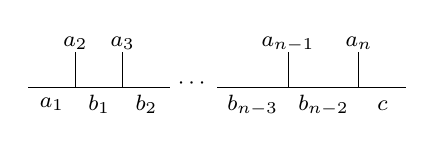
\begin{tikzpicture}[scale=0.3,font=\footnotesize,anchor=mid,baseline={([yshift=-.5ex]current bounding box.center)}]
    \node at (0, -0.6) {$a_1$};
    \node at (1, 2) {$a_2$};
    \node at (3, 2) {$a_3$};
    \node at (10, 2) {$a_{n-1}$};
    \node at (13, 2) {$a_n$};
%
    \draw (1, 0) to (1, 1.5);
    \draw (3, 0) to (3, 1.5);
%
    \draw (10, 0) to (10, 1.5);
    \draw (13, 0) to (13, 1.5);
%
    \draw (-1, 0) to (5, 0);
    \draw (7, 0) to (15, 0);
%
    \node at (2, -0.7) {$b_1$};
    \node at (4, -0.7) {$b_2$};
    \node at (6, 0.2) {$\cdots$};
%
    \node at (8.5, -0.7) {$b_{n-3}$};
    \node at (11.5, -0.7) {$b_{n-2}$};
    \node at (14, -0.7) {$c$};
  \end{tikzpicture}
  \;\;\;\bigg|\; \begin{array}{c}\text{for all possible intermediate} \\ \text{charges $b_1, b_2, \ldots, b_{n-2}$}\end{array}
  \right\}.
\end{align*}
We can thus think of the basis as consisting of a tuples of possible intermediate charges
\begin{align*}
  (b_1, b_2, \ldots, b_{n-2}).
\end{align*}

TODO: Mention coordinatization, i.e. representing all this with $\mathbb{C}^n$ matrices.

The real advantage of writing fusions states with fusion diagrams is that braiding is much easier to represent. This will be extremely useful now as we proceed in developing the abstract model for anyons, and characterize braiding.


\section{The $R$-matrix: Commutativity of fusion}

The result of fusing $a$ with $b$ must be the same as fusing $b$ with $a$. That is, fusion is commutative,
\begin{align*}
  a \times b = b \times a.
\end{align*}
This gives rise to a natural isomorphism
\begin{align*}
  R : V_{ba}^c \to V_{ab}^c
\end{align*}
between the corresponding fusion spaces % $V_{ab}^c \cong V_{ba}^c$,
which can be represented by a unitary matrix $R_{ab}^c$ in the canonical basis
\begin{align*}
  \ket{ba,c,\mu} = \sum_{\mu'} (R_{ab}^c)_{\mu}^{\mu'} \ket{ab,c,\mu'}.
\end{align*}
As we have seen, if the fusion multiplicities $N_{ab}^c \le 1$ for all labels $a,b,c$, we can disregard explicit mention of the fusion multiplicities. From now on we shall do so, and note that it is straight forward to add these indices back if needed. In the diagrammatic notation we then have
\begin{equation}\label{R-matrix}
  \fsfusedbraided{}{a}{b}{}{c} = R_{ab}^c \fsfused{}{a}{b}{}{c}.
\end{equation}
In this case it is clear that $R$-matrix $R_{ab}$ is diagonal in the canonical basis and we have
\begin{align*}
  (R_{ab})_{ij} = \delta_{ij} R_{ab}^i.
\end{align*}

\section{The $F$-matrix: Associativity of fusion}

The result of fusing multiple anyons must be independent of which anyons are fused first. That is, fusion is associative,
\begin{align*}
  (a \times b) \times c = a \times (b \times c)
\end{align*}
This gives rise to a natural isomorphism between the two decompositions of the fusion space
\begin{align*}
  V_{abc}^d \cong
  \bigoplus_f V_{ab}^f \otimes V_{fc}^d
  \cong
  \bigoplus_e V_{bc}^e \otimes V_{ae}^d
  .
\end{align*}
The first decomposition should be understood as first fusing $a$ with $b$ in all possible ways giving an intermediate charge $f$, followed by fusing $c$ with $f$ to give the final charge $d$.
The second decomposition should be understood as first fusing $b$ with $c$ in all possible ways giving an intermediate charge $e$, followed by fusing $a$ with $e$ to give the final charge $d$.

The first of these two decompositions is referred to as the standard decomposition and the second is the fusion decomposition. We denote this isomorphism by
\begin{align*}
  F : \bigoplus_f V_{ab}^f \otimes V_{fc}^d \to \bigoplus_e V_{bc}^e \otimes V_{ae}^d
\end{align*}
and it can be represented by the matrix $F_{abc}^c$, satisfying the equation
\begin{equation}\label{F-matrix}
  \sum_f \left(F_{abc}^d\right)_{ef} \fs{b,c}{a,f,d} = \fsfused{a}{b}{c}{d}{e}.
\end{equation}
That is, the $F$-matrix is the change of basis matrix from the standard basis to the fusion basis of the fusion space $V_{abc}^d$.

The following lemma will be useful when computing the $F$-matrix.

\begin{lemma}\label{res:F1}
  Consider the fusion space $V_{abc}^d$, when one of the particle types is trivial, i.e. $a,b,c$ or $d$ equals $1$, then $\dim V_{abc}^d = 1$ and the corresponding $F$-matrix $F_{abc}^d$ is trivial. More explicitly we have
  \begin{align*}
    F_{1bc}^d &= \left( F_{1bc}^d \right)_{db} = 1, \\
    F_{a1c}^d &= \left( F_{a1c}^d \right)_{ca} = 1, \\
    F_{ab1}^d &= \left( F_{ab1}^d \right)_{bd} = 1, \\
    F_{abc}^1 &= \left( F_{abc}^1 \right)_{\overline{a}\,\overline{c}} = 1.
  \end{align*}
\end{lemma}

\begin{proof}
  With $a = 1$ we have, by definition of the $F$-matrix,
  \begin{align*}
     \fsfused{1}{b}{c}{d}{e} = \sum_f \left(F_{1bc}^d \right)_{ef} \fs{b,c}{1,f,d}.
  \end{align*}
  From the fusion diagram on the right hand side we read out $1 \times b = f$ from the first fusion, this is valid only for $b = f$.
  Similarly, on the left hand side the final fusion reads $1 \times e = d$, implying $e = d$. Since the indices $e$ and $f$ are forced, this implicitly shows that the corresponding fusion spaces is one-dimensional. The other results follow analogously,
  \begin{align*}
    % \fs{b,c}{a,e,d} &= \sum_f \left(F_{abc}^d \right)_{ef} \fsfused{a}{b}{c}{d}{f} \\
    \fsfused{a}{1}{c}{d}{e} &= \sum_f \left(F_{a1c}^d \right)_{ef} \fs{1,c}{a,f,d} \implies e = c, f = a, \\
    \fsfused{a}{b}{1}{d}{e} &= \sum_f \left(F_{ab1}^d \right)_{ef} \fs{b,1}{a,f,d} \implies e = b, f = d, \\
    \fsfused{a}{b}{c}{1}{e} &= \sum_f \left(F_{abc}^1 \right)_{ef} \fs{b,c}{a,f,1} \implies e = \overline{a}, f = \overline{c}.
  \end{align*}
  The result can also be realized by noting that three anyons of type $a, b$ and $c$, where one of them is the trivial type $1$, is uniquely determined by their total charge. Indeed, these three anyons are really just two, since the trivial particle $q$ fuses trivially, it can be added or removed in the representation without changing anything. Thus, the corresponding $F$ matrix must be trivial in this case.
\end{proof}



\section{The $B$-matrix: Braiding of basic fusion states}

We shall now consider braiding on the standard fusion states. This can be realized by applying the $F$-matrix to put the state in a basis where the $R$ matrix can be applied immediately, followed by reverting back to the standard basis via $F^{-1}$. That is, using the $F$ and $R$-matrix we obtain the relation
% \begin{align*}
%   \fs[1]{b,c}{a,e,d}
%   &= \sum_f \left(F_{acb}^d\right)_{ef} \fsfusedbraided{a}{b}{c}{d}{f} \\
%   &= \sum_f \left(F_{acb}^d\right)_{ef} R_{bc}^f \fsfused{a}{b}{c}{d}{f} \\
%   &= \sum_g \sum_f \left(F_{acb}^d\right)_{ef} R_{bc}^f \left((F^{-1})_{abc}^d\right)_{fg} \fs{b,c}{a,g,d}.
% \end{align*}
\begin{align*}
  \fs[1]{b,c}{a,e,d}
  &= \sum_f \left(\left(F^{-1}\right)_{acb}^d\right)_{ef} \fsfusedbraided{a}{b}{c}{d}{f} \\
  &= \sum_f \left(\left(F^{-1}\right)_{acb}^d\right)_{ef} R_{bc}^f \fsfused{a}{b}{c}{d}{f} \\
  &= \sum_g \sum_f \left(\left(F^{-1}\right)_{acb}^d\right)_{ef} R_{bc}^f \left(F_{abc}^d\right)_{fg} \fs{b,c}{a,g,d}.
\end{align*}
From this we define the $B$-matrix as
\begin{align*}
  \left(B_{abc}^d\right)_{eg} = \sum_f \left(F_{acb}^d\right)_{ef} R_{bc}^f \left((F^{-1})_{abc}^d\right)_{fg},
\end{align*}
which braids the standard fusion states according to
\begin{align*}
  \fs[1]{b,c}{a,e,d} = \sum_g \left(B_{abc}^d\right)_{eg} \fs{b,c}{a,g,d}.
\end{align*}

TODO: I'm confused about Preskill's convention, $F$ and $F^{-1}$ end up interchanged. However, I do get the same as \cite{bonderson}.
% This leads to wrong expression for $FRF^{-1} = \rho(\sigma_2) \ne F^{-1}RF$. However $F = F^{-1}$ for Fibonacci anyons, so this error is not immediately detected. But still an error in the general setting.

As a consequence of the definition of the $B$-matrix and \cref{res:F1} we have the following lemma, which will be useful when computing the $B$-matrix.

\begin{lemma}\label{res:B1}
  Consider the fusion space $V_{abc}^d$, when one of the particle types is trivial, i.e. $a,b,c$ or $d$ equals $1$, then $\dim V_{abc}^d = 1$ and the corresponding $B$-matrix $B_{abc}^d$ is one-dimensional,
  \begin{align*}
    B_{1bc}^d &= \left( B_{1bc}^d \right)_{c b} = R_{bc}^d, \\
    B_{a1c}^d &= \left( B_{a1c}^d \right)_{d a} = R_{1c}^c, \\
    B_{ab1}^d &= \left( B_{ab1}^d \right)_{a d} = R_{b1}^b, \\
    B_{abc}^1 &= \left( B_{abc}^1 \right)_{\overline{b} \overline{c}} = R_{bc}^{\overline{a}}.
  \end{align*}
\end{lemma}



\section{Braid group representations $\rho(\sigma_j)$: Braiding of general fusion states}\label{sec:general braiding}

Consider the fusion space $V_{a_1 \cdots a_n}^c$ in a given anyon model, the representation $\rho(\sigma_j)$ gives the anyonic phase introduced to the total wave function when particles $a_j$ and $a_j+1$ are exchanged (counter)clockwise. Recall from TODO that the braid group is generated by $\sigma_1, \ldots, \sigma_n$, thus it suffices to give expressions for $\rho(\sigma_j)$ in order to be able to compute any braid in a given anyon model.
% Computing the representations $\rho(\sigma_j)$ of the generators in the general case will thus be of paramount importance.

Before showing how $\rho(\sigma_j)$ is computed, we begin by making our notation slightly more flexible. Consider the fusion space $V_{a_1\ldots a_n}^c$. As we have seen, the fusion states are on the form
\begin{align*}
  \fswide{a_2,a_3}{a_1,b_1,b_2} \ldots \fswider{a_{n-1},a_n}{b_{n-3},b_{n-2},c}.
\end{align*}
We shall sometimes write such states on the form of the standard basis states of $V_{1a_1\ldots a_n}^c$, i.e. as
\begin{align*}
  \fswide{a_1,a_2}{1,a_1,b_1} \ldots \fswider{a_{n-1},a_n}{b_{n-3},b_{n-2},c}.
\end{align*}
The reason being that it is then simpler to represent braiding of $a_1$ with $a_2$. This observation allows us to extend the fusion diagrams with trivial charges when convenient.

\begin{lemma}\label{res:sigma 1 is R}
  In a general anyon model, consider the fusion space $V_{a_1\cdots a_n}^c$ in the standard basis, then
  \begin{align*}
    \rho(\sigma_1)_{ij} = \delta_{ij} R_{a_1 a_2}^{j} \quad \iff \quad \rho(\sigma_1) = R_{a_1 a_2}.
  \end{align*}
\end{lemma}

\begin{proof}
  In the general case, the representation $\rho(\sigma_1)$ for the first generator $\sigma_1$ that braids $a_1$ with $a_2$, is given by
  \begin{align*}
    \rho(\sigma_1) \left( \fswide{a_1,a_2}{1,a_1,b_1} \ldots \right) = \left( \fswide[1]{a_1,a_2}{1,a_2,b_1} \ldots \right) = \sum_g \left[ \left(B_{1 a_1 a_2}^{b_1}\right)_{a_2 g} \left( \fswide{a_1,a_2}{1,g,b_1} \ldots \right)\right]
  \end{align*}
  Since $1$ fuses trivially we must have $g = a_1$ and thus $\rho(\sigma_1)$ is one-dimensional with
  \begin{align*}
    \rho(\sigma_1) = \left( B_{1 a_1 a_2}^{b_1} \right)_{a_2, a_1} = \sum_f \left( F_{1 a_2 a_1}^{b_1} \right)_{a_2 f} R_{a_1 a_2}^{f} \left( \left( F^{-1} \right)_{1 a_1 a_2}^{b_1} \right)_{f a_1} = R_{a_1 a_2}^{b_1},
  \end{align*}
  where the last equality follows from \cref{res:F1}.
\end{proof}

\begin{remark}
  Above, $\rho(\sigma_1)$ is expressed in the basis for the reduced space $V_{a_1 a_2} = \bigoplus_{b_1} V_{a_1 a_2}^{b_1}$, having basis determined by the possible anyonic labels $b_1$. Equivalently, in the basis for the full space $V_{a_1 \cdots a_n}^c$ we have
  \begin{align*}
    \rho(\sigma_1) = R_{a_1 a_2} \otimes \mathbbm{1}.
  \end{align*}
  The full space $V_{a_1 \cdots a_n}^c$ has basis states $(b_1,\ldots,b_{n-2})$ and we implicitly used the operator on the space reduced to fusion states $(b_1)$.
  For convenience, we shall abuse notation and not write this explicitly. It should always be clear what part of the space that the operator acts on.
\end{remark}

\begin{lemma}\label{res:sigma j is B}
  In a general anyon model, consider the fusion space $V_{a_1\cdots a_n}^c$ with the standard basis $(b_1,\ldots,b_{n-1})$, then
  \begin{align*}
    \rho(\sigma_j) = B_{b_{j-2} a_j a_{j+1}}^{b_j},
  \end{align*}
  % where we are abusing notation and letting it be implicit that $\rho(\sigma_j)$ acts on the part of the space that has the intermediate charge index $b_{j-1}$ free. Explicitly we have
  % \begin{align*}
  %   \rho(\sigma_j) \equiv \mathbbm{1}_{b_1,\ldots,b_{j-2}} \otimes \rho(\sigma_j) \otimes \mathbbm{1}_{b_j,\ldots,b_{j-2}}.
  % \end{align*}
\end{lemma}

\begin{proof}
  Note that $\rho(\sigma_j)$ is precisely the $B$-matrix applied appropriately,
  \begin{align*}
    \left( \ldots \fswider[1]{a_j,a_{j+1}}{b_{j-2},e,b_{j}} \ldots \right) = \sum_{b_{j-1}} \left[ \left(B_{b_{j-2} a_j a_{j+1}}^{b_{j}}\right)_{e, b_{j-1}} \left( \ldots \fswider{a_j,a_{j+1}}{b_{j-2},b_{j-1},b_{j}} \ldots \right) \right],
  \end{align*}
  thus the result follows.
\end{proof}

With the convention $b_{0} = a_1$ and $b_{-1} = 1$, \cref{res:sigma j is B} subsumes \cref{res:sigma 1 is R}, and also the following result, which we state explicitly for convenience. Recall that $\overline{a}$ denotes the antiparticle of $a$.

\begin{lemma}\label{res:sigma n-1 is R}
  In a general anyon model, consider the fusion space $V_{a_1\cdots a_n}^1$ with its standard basis $(b_1, \ldots, b_{n-3})$ (note that $c=1$ forces $b_{n-2} = \overline{a_n}$), then
  \begin{align*}
    \rho(\sigma_{n-1})_{ij} = \delta_{ij} R_{a_{n-1} a_n}^{\overline{j}},
  \end{align*}
  acting on the $b_{n-3}$-part of the space.
\end{lemma}

\begin{proof}
  Since the result of the fusion is assumed to be the trivial particle $1$, we must have the indices as follows,
  \begin{gather*}
    \rho(\sigma_{n-1}) \left( \ldots \fswider{a_{n-1},a_n}{b_{n-3},\overline{a_n},1} \right)
    = \left( \ldots \fswider[1]{a_{n-1},a_n}{b_{n-3},\overline{a_{n-1}},1} \right) \\
    = \sum_g \left[ \left(B_{b_{n-3} a_{n-1} a_n}^{1}\right)_{\overline{a_{n-1}}, g} \left( \ldots \fswider{a_{n-1},a_n}{b_{n-3},g,1} \right) \right].
  \end{gather*}
  Since the last fusion reads $g \times a_n = 1$ we must have $g = \overline{a_n}$ and thus
  \begin{align*}
    \rho(\sigma_{n-1}) &= \left( B_{b_{n-3} a_{n-1} a_n}^{1} \right)_{\overline{a_{n-1}}, \overline{a_n}} \\
    &= \sum_f \left( F_{b_{n-3} a_n a_{n-1}}^1 \right)_{\overline{a_{n-1}} f} R_{a_{n-1} a_n}^f \left( \left( F^{-1} \right)_{b_{n-3} a_{n-1} a_n}^1 \right)_{f,\overline{a_n}} \\
    &= R_{a_{n-1} a_n}^{\overline{b_{n-3}}}
  \end{align*}
  where the last equality follows from \cref{res:F1}.
\end{proof}

\begin{remark}
  Note that $\rho(\sigma_1)$ and $\rho(\sigma_{n-1})$ are equal in the restricted basis, up to charge conjugation of the basis. Furthermore, note that if time is reversed, the roles of $\rho(\sigma_1)$ and $\rho(\sigma_j)$ are interchanged. Reversing the fusion in time means reading the fusion diagram from right/bottom to left/top. This is an example of time reversal symmetry; time reversal corresponds to charge conjugation, see \cite{nayak}.
\end{remark}

Time reversal as charge conjugation is also simply manifested in the following lemma, as a result of \cref{res:sigma 1 is R} and \ref{res:sigma n-1 is R}.
\begin{lemma}
  In the standard basis the $R$ matrix can be written as
  \begin{align*}
    \fsfusedbraided{}{a}{b}{}{c} = R_{ab}^c \fsfused{}{a}{b}{}{c}
    \quad \iff \quad
    \fs[1]{a,b}{1,b,c} = R_{ab}^c \fs{a,b}{1,a,c}
    \quad \iff \quad
    \fs[1]{a,b}{c,\overline{a},1} = R_{ab}^{\overline{c}} \fs{a,b}{c,\overline{b},1}.
  \end{align*}
\end{lemma}



\section{The pentagon and hexagon equations}

When considering an anyon model, it is ultimately the $B$-matrix that determines the properties of interest. The $B$-matrix gives the phase change introduced by exchanging pairs of anyons, i.e. braiding. In the previous section we saw how the $B$-matrix determine the braid group representation. This is the relevant property both for the study the dynamics of anyons, but also for developing methods for quantum computation with anyons, known as topological quantum computation.

We have seen that the $B$-matrix is computed from the $F$ and $R$-matrices. These matrices are in turn determined by what is known as the pentagon equation
\begin{equation}\label{eq:pentagon}
  \left(F_{12c}^5\right)^d_a \left(F_{a34}^5\right)^c_b = \left(F_{234}^d\right)_c^c \left( F_{1e4}^5 \right)^d_b \left( F_{123}^b \right)^e_a
\end{equation}
and hexagon equation
\begin{equation}\label{eq:hexagon}
  R_{13}^c \left(F_{213}^4\right)^c_a R_{12}^a = \sum_{b} \left(F_{231}^4\right)^c_b R_{1b}^4 \left(F_{123}^4\right)^b_a.
\end{equation}
In these equations, all indices are taken as arbitrary particle labels.

These equations are known as coherence conditions for fusion and braiding. The diagrammatic version of these equations, found as commutative diagrams in \cref{fig:pentagon_diagram,fig:hexagon_space} and \cref{fig:pentagon_space,fig:hexagon_space} make the point clearer, and shows that these equations are commutativity constraints for fusion and braiding. Indeed, the pentagon equation is the formal constraint for associativity of fusion,
\begin{align*}
  (a \times b) \times c = a \times (b \times c).
\end{align*}
As previously hinted, anyon models can be described by braided tensor categories. In this setting, the pentagon and hexagon equations are precisely Mac Lane's coherence theorem \cite{mac lane}, showing that no further conditions are required for consistent fusion and braiding. Further details can be found in \cite{kitaev,preskill}.

Solving the pentagon and hexagon equations is in general highly non-trivial. The equations are multivariate polynomial equations and require elaborate techniques to be solved. First one must fix the gague freedom that comes from the choice of basis for the fusion space, next an appropriate Gröbner basis can be used to solve the system. See \cite{bonderson} for more details.

\begin{figure}[h]
  \centering
  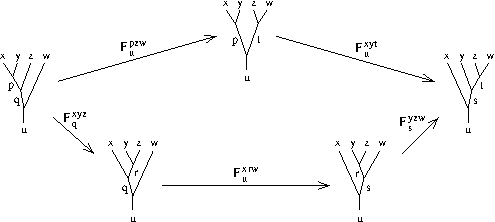
\includegraphics[width=1\linewidth]{img/pentagon_diagram.pdf}
  \caption{The pentagon equation in terms of fusion diagrams. Figure take from \cite{kitaev}. Note that the $F$-matrix have super- and sub-scripts reversed.}
  \label{fig:pentagon_diagram}
\end{figure}

\begin{figure}[h]
  \centering
  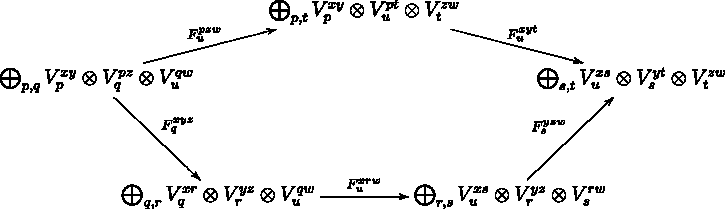
\includegraphics[width=1\linewidth]{img/pentagon_space.pdf}
  \caption{The pentagon equation in terms of fusion spaces. Figure take from \cite{kitaev}. Note that the fusion spaces and the $F$-matrix have super- and sub-scripts reversed.}
  \label{fig:pentagon_space}
\end{figure}


\begin{figure}[h]
  \centering
  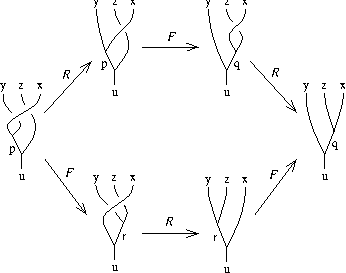
\includegraphics[width=0.8\linewidth]{img/hexagon_diagram.pdf}
  \caption{The hexagon equation in terms of fusion diagrams. Figure take from \cite{kitaev}.}
  \label{fig:hexagon_diagram}
\end{figure}

\begin{figure}[h]
  \centering
  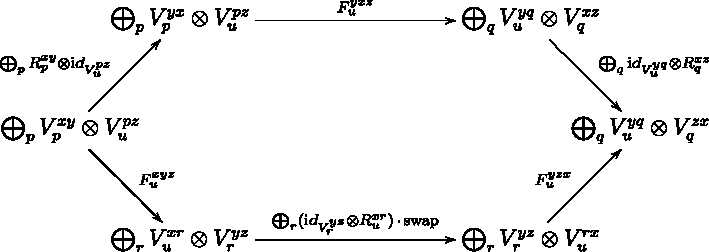
\includegraphics[width=1\linewidth]{img/hexagon_space.pdf}
  \caption{The hexagon equation in terms of fusion spaces. Figure take from \cite{kitaev}. Note that the fusion spaces, $F$-matrix and $R$-matrix have super- and sub-scripts reversed.}
  \label{fig:hexagon_space}
\end{figure}


\clearpage































\chapter{Fibonacci anyons}\label{fibonacci anyons}

The Fibonacci anyon model is the simples non-Abelian anyon model, yet containing all the interesting features of non-Abelian anyons. Another common model is the Ising model, however Ising anyons cannot be used for general quantum computation.

This chapter is partly based on \cite{preskill} and \cite{topological quantum compiling}. The literature is rather vague on deriving the properties of Fibonacci anyons, in this chapter we spelled out the details more clearly.

\section{Preliminaries}

The Fibonacci anyon model consists of two particle types, $1$ (the mandatory trivial particle type) and $\tau$ (non-trivial) with the corresponding fusion rules
\begin{align*}
  1 \times 1 = 1, \quad
  1 \times \tau = \tau, \quad
  \tau \times \tau = 1 + \tau.
\end{align*}

The following observation motivates the name of the model. Consider the fusion spaces $V_{\tau^n}^1$, where $\tau^n$ denotes $n$ repetitions of $\tau$. This is the space of possible fusions of $n$ Fibonacci anyons, having total charge $1$. Writing out the canonical basis for these spaces we find
\begin{align*}
  V_{\tau\tau}^1 &:
    \left\{
      \fs{\tau,\tau}{1,\tau,1}
    \right\} \\
  V_{\tau\tau\tau}^1 &:
    \left\{
      \fs{\tau,\tau,\tau}{1,\tau,\tau,1}
    \right\} \\
  V_{\tau\tau\tau\tau}^1 &:
    \left\{
      \fs{\tau,\tau,\tau,\tau}{1,\tau,\boldsymbol{1},\tau,1},
      \fs{\tau,\tau,\tau,\tau}{1,\tau,\boldsymbol{\tau},\tau,1}
    \right\} \\
  V_{\tau\tau\tau\tau\tau}^1 &:
    \left\{
      \fs{\tau,\tau,\tau,\tau,\tau}{1,\tau,\boldsymbol{1},\boldsymbol{\tau},\tau,1},
      \fs{\tau,\tau,\tau,\tau,\tau}{1,\tau,\boldsymbol{\tau},\boldsymbol{1},\tau,1},
      \fs{\tau,\tau,\tau,\tau,\tau}{1,\tau,\boldsymbol{\tau},\boldsymbol{\tau},\tau,1}
    \right\} \\
  V_{\tau\tau\tau\tau\tau\tau}^1 &:
    \left\{
      \fs{\tau,\tau,\tau,\tau,\tau,\tau}{1,\tau,\boldsymbol{1},\boldsymbol{\tau},\boldsymbol{1},\tau,1},
      \fs{\tau,\tau,\tau,\tau,\tau,\tau}{1,\tau,\boldsymbol{1},\boldsymbol{\tau},\boldsymbol{\tau},\tau,1},
      \fs{\tau,\tau,\tau,\tau,\tau,\tau}{1,\tau,\boldsymbol{\tau},\boldsymbol{\tau},\boldsymbol{1},\tau,1}
      \fs{\tau,\tau,\tau,\tau,\tau,\tau}{1,\tau,\boldsymbol{\tau},\boldsymbol{1},\boldsymbol{\tau},\tau,1},
      \fs{\tau,\tau,\tau,\tau,\tau,\tau}{1,\tau,\boldsymbol{\tau},\boldsymbol{\tau},\boldsymbol{\tau},\tau,1}
    \right\}.
\end{align*}
The reader can continue this list. Note that the bottom line in the fusion diagrams of the fusion states in the bases can be seen as strings of $\tau$ and $1$, having $1\tau$ at the start and $\tau 1$ at the end. Furthermore, the string is subject to the condition that $1$ may not be followed by $1$. Indeed, $1$ on the bottom row, fuses with $\tau$ from the top, to give $\tau$. It is thus clear that
\begin{align*}
  \dim V_{\tau^n}^1 = \operatorname{Fib}(n-1)
\end{align*}
where $\operatorname{Fib}(n)$ denotes the $n$:th Fibonacci number. That is, the dimension of the fusion space grows with increasing number of $\tau$s as the Fibonacci series.

As we have seen in \label{anyon models}, an anyon model is determined by the corresponding $F$- and $R$-matrices. We continue by computing these matrices.


% TODO: Motivate Fibonacci name. $\dim(V_{\tau^n}^\tau) = \Fib(n)$
% By the product rule for quantum dimensions \eqref{eq:quantum dimension product rule} we have
% \begin{align*}
%   d_1^2 &= d_1 \implies d_1 = 1 \\
%   d_\tau^2 &= \tau + d_\tau \implies d_\tau = \varphi
% \end{align*}
% where $\varphi = \frac{1+\sqrt{5}}{2}$ is the golden ratio. Furthermore, the series $(d_1(n))_n$ is the Fibonacci series.




\section{Determining the model: Computing the $F$ and $R$-matrices}

TODO: This section must be cleaned up! Ignore the text below

The $F$-matrix is determined by solving the pentagon equation. This is in general highly non-trivial, but for the case of Fibonacci anyons this is rather straight forward. In order to simplify the calculations we make the observation that $F_{abc}^d = 1$, i.e. fusion acts trivially when there is just two non-trivial charges involved in the fusion. Thus, it remains to determine $F_{\tau\tau\tau}^1$ and $F_{\tau\tau\tau}^\tau$. We make a second observation, namely
\begin{align*}
  (F_{\tau\tau\tau}^1)_{ab} = \delta_{a\tau}\delta_{b\tau},
\end{align*}
since $\tau$ is the only allowed intermediate charge when three Fibonacci anyons fuse to the vacuum. Next

\cite[p. 389-390]{short intro fib} argues that the only non-trivial $F$-matrix is $F^{\tau\tau\tau}_\tau \eqqcolon F$.
Since $F$ is unitary, $FF^* = I$, it can be written on the form
\begin{equation*}
  F = \begin{pmatrix} a & b \\ -e^{i\theta}b^* & e^{i\theta}a^* \end{pmatrix}
\end{equation*}
for $\theta \in [0, 2\pi)$ and $a, b \in \mathbb{C}$ such that $|a|^2 + |b|^2 = 1$.
Furthermore, $F$ is its own inverse. (This is clear from the diagrammatic representation of $F$, since reversing the order of fusion twice takes us back to the initial order of fusion. TODO: Show this from nPOV). Thus
\begin{equation*}
  F = F^*
  \iff
  \begin{pmatrix} a & b \\ -e^{i\theta}b^* & e^{i\theta}a^* \end{pmatrix}
  =
  \begin{pmatrix} a^* & -e^{-i\theta}b \\ b^* & e^{-i\theta}a^* \end{pmatrix}.
\end{equation*}
Equality for the first element shows that $a \in R$, equality for the second and third element give the same condition, namely $-e^{i\theta} = 1$, that is $\theta = \pi$. Finally, equality for the fourth element gives no more information. Thus,
\begin{equation*}
  F = \begin{pmatrix} a & b \\ b^* & -a \end{pmatrix}.
\end{equation*}
Let $F$ be expressed in the $\{1, \tau\}$ basis, The pentagon equation then reduces to
\begin{equation*}
  F_{1,1} = F_{1,\tau} F_{\tau,1} \iff a = |b|^2 \quad (\implies a \ge 0).
\end{equation*}
The unitarity condition $|a|^2 + |b|^2 = 1$ thus reduces to
\begin{equation*}
  a^2 + a = 1, a \ge 0 \iff a = \varphi^{-1}
\end{equation*}
where $\varphi = \frac{1+\sqrt{5}}{2}$ is the golden ratio. Finally, $a = |b|^2 \implies b = e^{i\phi}\varphi^{-1/2}$, where the phase $\phi$ is arbitrary and by a suitable phase convention can be set to zero TODO: Why?. Hence
\begin{equation*}
  F = \begin{pmatrix} \varphi^{-1} & \varphi^{-1/2} \\ \varphi^{-1/2} & -\varphi^{-1} \end{pmatrix}
\end{equation*}

TODO: Introduce $R$ matrices. Calculate $R$ for fib. anyons. Then generators of $B$ are $\sigma_1 = R, \sigma = F^{-1}RF$. Compare this to the other representation of $B$.


\hrule

The only non-trivial $F$-matrix is $F_{\tau\tau\tau}^\tau$, which is two-dimensional. By considering the valid fusion channels for $F_{\tau\tau\tau}^1$,
\begin{align*}
  \fs{\tau,\tau}{\tau,e,1} = \sum_f \left(F_{\tau\tau\tau}^1\right)_e^f \fsfused{\tau}{\tau}{\tau}{1}{f}
\end{align*}
we see that only $e=f=\tau$ correspond to valid fusions, thus $\left(F_{\tau\tau\tau}^1\right)_\tau^\tau$ acts trivially. With the same argument applied to the remaining $F$-matrices we obtain
\begin{alignat*}{100}
  % 1 =
  \left(F_{1\tau\tau}^\tau\right)_\tau^\tau &{}={}&
  \left(F_{\tau1\tau}^\tau\right)_\tau^\tau &{}={}&
  \left(F_{\tau\tau1}^\tau\right)_\tau^\tau &{}=
  \\
  \left(F_{11\tau}^\tau\right)_1^\tau &{}={}&
  \left(F_{1\tau1}^\tau\right)_\tau^\tau &{}={}&
  \left(F_{\tau11}^\tau\right)_\tau^1 &{}=
  \\
  \left(F_{1\tau\tau}^1\right)_\tau^1 &{}={}&
  \left(F_{\tau1\tau}^1\right)_\tau^\tau &{}={}&
  \left(F_{\tau\tau1}^1\right)_1^\tau &{}=
  \\
  \left(F_{\tau\tau\tau}^1\right)_\tau^\tau &{}={}&
  \left(F_{111}^1\right)_1^1&=1\hspace{-2em}
\end{alignat*}
Other indices correspond to invalid fusions, and the corresponding $F$-matrices never show up in computations since there is no fusion state on which they act.


For convenience, when discussing Fibonacci anyons, let
\begin{align*}
  F \coloneqq F_{\tau\tau\tau}^\tau, &&
  R \coloneqq R_{\tau\tau}, &&
  B \coloneqq FRF^{-1}.
\end{align*}



\section{Braiding of Fibonacci anyons}

In this section we shall compute the braid group generators for various number of Fibonacci anyons. Ultimately, we shall compute $\rho(\sigma_j)$ for $V_{\tau^n}^1$. Having trivial total charge represents the fact that we have exactly $n$ anyons. If the total charge would be $\tau$, there would really be $n+1$ Fibonacci anyons available. As we shall see, there will be some subtleties regarding different charge sectors, i.e. different total charge, when considering braiding of intermediate $\tau$ anyons in $V_{\tau^n}^1$. We begin with some elementary examples.

Recall the notation
\begin{align*}
  V_{a_1\cdots a_n} = \bigoplus_{c} V_{a_1 \cdots a_n}^c
\end{align*}
then, in particular
\begin{align*}
  V_{\tau^n} = V_{\tau^n}^1 \oplus V_{\tau^n}^\tau.
\end{align*}


\subsection{Braiding in $V_{\tau^2}$}

The two charge sectors of $V_{\tau^2}$ have the standard basis
\begin{align*}
  V_{\tau\tau}^1    = \operatorname{span} \left\{ \fs{\tau,\tau}{1,\tau,\boldsymbol{1}} \right\}, \quad
  V_{\tau\tau}^\tau = \operatorname{span} \left\{ \fs{\tau,\tau}{1,\tau,\boldsymbol{\tau}} \right\}.
\end{align*}
That is, the fusion space $V_{\tau^2}$ is two-dimensional. Since there is only two $\tau$-anyons, there are only one generator for the braid group, $\sigma_1$. We compute $\rho(\sigma_1)$ by considering its action on the standard fusion states,
\begin{align*}
  \rho(\sigma_1) \fs{\tau,\tau}{1,\tau,1}    &= \fs[1]{\tau,\tau}{1,\tau,1}    = R_{\tau\tau}^1    \fs{\tau,\tau}{1,\tau,1} \\
  \rho(\sigma_1) \fs{\tau,\tau}{1,\tau,\tau} &= \fs[1]{\tau,\tau}{1,\tau,\tau} = R_{\tau\tau}^\tau \fs{\tau,\tau}{1,\tau,\tau}.
\end{align*}
Thus we have
\begin{align*}
  \left.\begin{aligned}
    \rho(\sigma_1)_{11} &= R_{\tau\tau}^1 \\
    \rho(\sigma_1)_{1\tau} &= 0 \\
    \rho(\sigma_1)_{\tau\tau} &= R_{\tau\tau}^\tau \\
    \rho(\sigma_1)_{\tau1} &= 0
  \end{aligned}\right\}
  \quad\iff\quad
  \rho(\sigma_1) =
  \begin{pmatrix}
    R_{\tau\tau}^1 & 0 \\
    0 & R_{\tau\tau}^\tau
  \end{pmatrix}.
\end{align*}
This also follows immediately from \cref{res:sigma 1 is R}.

\subsection{Braiding in $V_{\tau^3}$}

The two charge sectors of $V_{\tau^3}$ have the standard basis
\begin{align*}
  V_{\tau\tau\tau}^1    = \operatorname{span} \left\{ \fs{\tau,\tau,\tau}{1,\tau,\boldsymbol{\tau},\boldsymbol{1}} \right\}, \quad
  V_{\tau\tau\tau}^\tau = \operatorname{span} \left\{ \fs{\tau,\tau,\tau}{1,\tau,\boldsymbol{1},\boldsymbol{\tau}}, \fs{\tau,\tau,\tau}{1,\tau,\boldsymbol{\tau},\boldsymbol{\tau}} \right\}.
\end{align*}
That is, the fusion space $V_{\tau^3}$ is three-dimensional, and we denote the ordered basis as $\{\tau1, 1\tau, \tau\tau\}$ Since there are three $\tau$-anyons, there are two generators for the braid group, $\sigma_1$ and $\sigma_2$.

\Cref{res:sigma 1 is R} gives
\begin{align*}
  \rho(\sigma_1)_{(\tau1),(\tau1)} &= R_{\tau\tau}^\tau \\
  \rho(\sigma_1)_{(1\tau),(1\tau)} &= R_{\tau\tau}^1 \\
  \rho(\sigma_1)_{(\tau\tau),(\tau\tau)} &= R_{\tau\tau}^\tau \\
  \rho(\sigma_1)_{i,j} &= 0 \text{ for } i \ne j.
\end{align*}
In matrix form that is
\begin{align*}
  \rho(\sigma_1) =
  \begin{pmatrix}
    R_{\tau\tau}^\tau \\
    & R_{\tau\tau}^1 \\
    & & R_{\tau\tau}^\tau
  \end{pmatrix}
  = R_{\tau\tau}^\tau \oplus R.
\end{align*}

\Cref{res:sigma n-1 is R} gives
\begin{align*}
  \rho(\sigma_2)_{(\tau1),(\tau1)} &= R_{\tau\tau}^\tau.
\end{align*}
We compute $\rho(\sigma_2)$ for the $\tau$-charge sector by considering its action on the standard fusion states
\begin{align*}
  \rho(\sigma_2) \fs{\tau,\tau,\tau}{1,\tau,1,\tau}    &= \fs[2]{\tau,\tau,\tau}{1,\tau,1,\tau}    = \left( B_{\tau\tau\tau}^\tau \right)_{11} \fs[2]{\tau,\tau,\tau}{1,\tau,1,\tau} + \left( B_{\tau\tau\tau}^\tau \right)_{1\tau} \fs[2]{\tau,\tau,\tau}{1,\tau,\tau,\tau}, \\
  \rho(\sigma_2) \fs{\tau,\tau,\tau}{1,\tau,\tau,\tau} &= \fs[2]{\tau,\tau,\tau}{1,\tau,\tau,\tau} = \left( B_{\tau\tau\tau}^\tau \right)_{\tau1} \fs[2]{\tau,\tau,\tau}{1,\tau,1,\tau} + \left( B_{\tau\tau\tau}^\tau \right)_{\tau\tau} \fs[2]{\tau,\tau,\tau}{1,\tau,\tau,\tau}.
\end{align*}
Thus we have
\begin{align*}
  \rho(\sigma_2)_{(1\tau),(1\tau)} &= \left(B_{\tau\tau\tau}^\tau\right)_{11} \\
  \rho(\sigma_2)_{(1\tau),(\tau\tau)} &= \left(B_{\tau\tau\tau}^\tau\right)_{1\tau} \\
  \rho(\sigma_2)_{(\tau\tau),(1\tau)} &= \left(B_{\tau\tau\tau}^\tau\right)_{\tau1} \\
  \rho(\sigma_2)_{(\tau\tau),(\tau\tau)} &= \left(B_{\tau\tau\tau}^\tau\right)_{\tau\tau}.
\end{align*}
In matrix form that is
\begin{align*}
  \rho(\sigma_2) =
  \begin{pmatrix}
    R_{\tau\tau}^\tau \\
    & B_{11} & B_{1\tau} \\
    & B_{\tau1} & B_{\tau\tau}
  \end{pmatrix}
  = R_{\tau\tau}^\tau \oplus B.
\end{align*}



\subsection{Braiding in $V_{\tau^4}^1$}

Consider $V_{\tau\tau\tau\tau}^1$, this is the smallest non-trivial proper fusion space having dimension two. The fusion space is proper in the sense that the there is only one charge sector and it is the trivial (vacuum) charge sector. That is, there are really only $4$ Fibonacci anyons. We shall compute the corresponding braid group representation determined by exchange of Fibonacci anyons in the standard basis of $V_{\tau\tau\tau\tau}^1$.

\begin{proposition}
  Consider four Fibonacci anyons with total anyonic charge $1$, i.e. consider $V_{\tau\tau\tau\tau}^1$ in the standard basis. Then, the representation of the braid generators are
  \begin{align*}
    \rho(\sigma_1) = R,\quad
    \rho(\sigma_2) = B,\quad
    \rho(\sigma_3) = R.
  \end{align*}
\end{proposition}

\begin{proof}
  % We shall follow the general procedure outlined in \cref{sec:general braiding}, i.e. we shall compute the action of the braid group generators on the standard fusions basis
  % \begin{align*}
  %   \left\{ \fs{\tau,\tau,\tau,\tau}{1,\tau,\tau,1,\tau,1}, \fs{\tau,\tau,\tau,\tau}{1,\tau,\tau,\tau,1} \right\} \equiv \{1, \tau\}.
  % \end{align*}
  % Note that we are actually working with the basis for $V_{1\tau\tau\tau\tau}^1$, these spaces are isomorphic because $1$ fuses trivially. This convention allows for a cleaner and more symmetric use of the diagram notation when performing braiding. This becomes important now that we compute the $B$-matrix.

  \Cref{res:sigma 1 is R} gives
  % \centermath{\begin{alignat*}{10}
  %   \rho(\sigma_1) \fs{\tau,\tau,\tau,\tau}{1,\tau,1,\tau,1}
  %   &=
  %   \fs[1]{\tau,\tau,\tau,\tau}{1,\tau,1,\tau,1}
  %   = \sum_{g=\tau} \left(B_{1 \tau \tau}^1\right)_{\tau}^g \fs{\tau,\tau,\tau,\tau}{1,g,1,\tau,1}
  %   = {} & \left(B_{1 \tau \tau}^1\right)_{\tau}^\tau & \fs{\tau,\tau,\tau,\tau}{1,\tau,1,\tau,1} &
  %   & {} + {} & 0 & \fs{\tau,\tau,\tau,\tau}{1,\tau,\tau,\tau,1} &
  %   \\
  %   \rho(\sigma_1) \fs{\tau,\tau,\tau,\tau}{1,\tau,\tau,\tau,1}
  %   &=
  %   \fs[1]{\tau,\tau,\tau,\tau}{1,\tau,\tau,\tau,1}
  %   = \sum_{g=\tau} \left(B_{1 \tau \tau}^\tau \right)_{\tau}^g \fs{\tau,\tau,\tau,\tau}{1,g,\tau,\tau,1}
  %   = {} & 0 & \fs{\tau,\tau,\tau,\tau}{1,\tau,1,\tau,1} &
  %   & {} + {} & \left(B_{1 \tau \tau}^\tau \right)_{\tau}^\tau & \fs{\tau,\tau,\tau,\tau}{1,\tau,\tau,\tau,1}, &
  % \end{alignat*}} \\
  % where both sums only run over the label $\tau$ because only this corresponds to a valid fusion.
  % Furthermore
  % \begin{align*}
  %   \left(B_{1 \tau \tau}^1\right)_{\tau}^\tau = R_{\tau\tau}^1, \quad
  %   \left(B_{1 \tau \tau}^\tau\right)_{\tau}^\tau = R_{\tau\tau}^\tau
  % \end{align*}
  % because $\left(F_{1\tau\tau}^1\right)_\tau^1 = \left(F_{1\tau\tau}^\tau\right)_\tau^\tau = 1$ and these are the only valid lables that occur in the sum of these $B$-matrices. Thus we have
  \begin{align*}
    \rho(\sigma_1) = B_{1\tau\tau}^{\tau} = R_{\tau\tau} =
    \begin{pmatrix}
      R_{\tau\tau}^1 & 0 \\
      0 & R_{\tau\tau}^\tau
    \end{pmatrix}.
  \end{align*}
  \Cref{res:sigma j is B} gives
  \begin{align*}
    \rho(\sigma_2)_{ij} = \left( B^\tau_{\tau\tau\tau} \right)_{ij} = \sum_f \left( F_{\tau\tau\tau}^\tau \right)_{if} R_{\tau\tau}^f \left( \left( F^{-1} \right)_{\tau\tau\tau}^\tau \right)_{fj}
  \end{align*}
  i.e.
  \begin{align*}
    \rho(\sigma_2) = F R F^{-1}.
  \end{align*}
  % \begin{align*}
  %   \rho(\sigma_2) \fs{\tau,\tau,\tau,\tau}{1,\tau,1,\tau,1}
  %   = \fs[2]{\tau,\tau,\tau,\tau}{1,\tau,1,\tau,1}
  %   &= \sum_g \left(B_{\tau \tau \tau}^\tau\right)_1^g \fs{\tau,\tau,\tau,\tau}{1,\tau,g,\tau,1} \\
  %   \rho(\sigma_2) \fs{\tau,\tau,\tau,\tau}{1,\tau,\tau,\tau,1}
  %   = \fs[2]{\tau,\tau,\tau,\tau}{1,\tau,\tau,\tau,1}
  %   &= \sum_g \left(B_{\tau \tau \tau}^\tau\right)_\tau^g \fs{\tau,\tau,\tau,\tau}{1,\tau,g,\tau,1} \\
  % \end{align*}
  % Thus,
  % \begin{align*}
  %   \left(\rho(\sigma_2)\right)_i^j = \left(B_{\tau \tau \tau}^\tau\right)_i^j = \sum_f (F_{\tau\tau\tau}^\tau)_i^f R_{\tau\tau}^f \left((F^{-1})_{\tau\tau\tau}^\tau\right)_f^j,
  % \end{align*}
  % that is,
  % \begin{align*}
  %   \rho(\sigma_2) = F R F^{-1}. % TODO: Fel i Preskill (9.127)
  % \end{align*}
  Finally, \cref{res:sigma n-1 is R} gives
  % \begin{align*}
  %   \rho(\sigma_3) \fs{\tau,\tau,\tau,\tau}{1,\tau,1,\tau,1}
  %   = \fs[3]{\tau,\tau,\tau,\tau}{1,\tau,1,\tau,1}
  %   &= \sum_g \left(B_{1 \tau \tau}^1\right)_\tau^g \fs{\tau,\tau,\tau,\tau}{1,\tau,g,\tau,1}
  %   = R_{\tau\tau}^1 \fs{\tau,\tau,\tau,\tau}{1,\tau,1,\tau,1},
  %   \\
  %   \rho(\sigma_3) \fs{\tau,\tau,\tau,\tau}{1,\tau,\tau,\tau,1}
  %   = \fs[3]{\tau,\tau,\tau,\tau}{1,\tau,\tau,\tau,1}
  %   &= \sum_g \left(B_{\tau \tau \tau}^1\right)_\tau^g \fs{\tau,\tau,\tau,\tau}{1,\tau,g,\tau,1}
  %   = R_{\tau\tau}^\tau \fs{\tau,\tau,\tau,\tau}{1,\tau,\tau,\tau,1}.
  % \end{align*}
  % which can also be written $\left(\rho(\sigma_3)\right)_i^j = \left(B_{i\tau\tau}^1\right)_\tau^j$. Note that $\rho(\sigma_1) = \rho(\sigma_3)$.
  \begin{align*}
    \rho(\sigma_3)_{ij} = \delta_{ij} R_{\tau\tau}^{\overline{j}}
    \iff
    \rho(\sigma_3) = R_{\tau\tau}
  \end{align*}
  since $\tau$ is its own antiparticle $\overline{\tau}$.
\end{proof}




\subsection{Braiding in $V_{\tau^n}^1$ the general case}

TODO When considering braiding of anyons, such as in \cite{topological quantum compiling}, we cannot restrict to a particular charge sector because TODO Similarly cannot restrict to $1$ on the left TODO make more explicit / describe better.


\subsection{Five Fibonacci anyons $V_{\tau^5}^1$}

Consider $V_{\tau^n}^1$ with the standard basis. Restrict attention to a pair of neighbouring $\tau$ anyons. Thus, we restrict attention to a part of the space with basis
\begin{align*}
  \left\{ \text{valid intermediate charges $abc$ in } \fs{\tau,\tau}{a,b,c} \right\} \equiv \{ 1\tau1, 1\tau\tau, \tau\tau1, \tau1\tau, \tau\tau\tau \}.
\end{align*}
From \cref{res:sigma j is B} we have
\begin{align*}
  \rho(\sigma_1) = B_{a\tau\tau}^c \quad\iff\quad \rho(\sigma_1)_{ij} = \left( B_{a\tau\tau}^c \right)_{ij}
\end{align*}
where the indices $i$ and $j$ run over the given basis element. In the above given order of the basis fusion states the $B$-matrix is block diagonal. That is, in the obvious identification of the fusion space with $\mathbb{C}^{5}$ we have
\begin{align*}
  \rho(\sigma_1) &=
  \begin{pmatrix}
    (B_{1\tau\tau}^1)_{\tau\tau} & & & & \\
    & (B_{1\tau\tau}^\tau)_{\tau\tau} & & & \\
    & & (B_{\tau\tau\tau}^1)_{\tau\tau} & & \\
    & & & (B_{\tau\tau\tau}^\tau)_{11} & (B_{\tau\tau\tau}^\tau)_{1\tau} \\
    & & & (B_{\tau\tau\tau}^\tau)_{\tau1} & (B_{\tau\tau\tau}^\tau)_{\tau\tau}
  \end{pmatrix} \\
  &=
  \begin{pmatrix}
    R_{\tau\tau}^1 & & & & \\
    & R_{\tau\tau}^\tau & & & \\
    & & R_{\tau\tau}^\tau & \\
    & & & (FRF^{-1})_{1 1} & (FRF^{-1})_{1 \tau} \\
    & & & (FRF^{-1})_{\tau 1} & (FRF^{-1})_{\tau \tau}
  \end{pmatrix} \\
  &= R \oplus R_{\tau\tau}^\tau \oplus B.
\end{align*}

Next, taking a third Fibonacci anyon $\tau$ into account and choosing the basis ordered as follows
\begin{gather*}
  \left\{ \text{valid intermediate charges $abcd$ in } \fs{\tau,\tau,\tau}{a,b,c,d} \right\} \equiv \\
  \{
      1 \tau\tau  1 , % definitely this first
%
      1 \tau  1 \tau,
      1 \tau\tau\tau,
%
    \tau  1 \tau  1 ,
    \tau\tau\tau  1 ,
%
    \tau  1 \tau\tau,
    \tau\tau\tau\tau,  % problem for \sigma_2
    \tau\tau  1 \tau, % problem for \sigma_2
  \}
\end{gather*}
we have
% \begin{alignat*}{10}
%   \rho(\sigma_1) &= R_{\tau\tau}^\tau &{}\oplus{}& R &{}\oplus{}& FRF^{-1} &{}\oplus{}& FRF^{-1} &{}\oplus{}& R_{\tau\tau}^\tau \\
%   \rho(\sigma_2) &= R_{\tau\tau}^\tau &{}\oplus{}& FRF^{-1} &{}\oplus{}& R &{}\oplus{}& R_{\tau\tau}^\tau &{}\oplus{}& J_2 FRF^{-1} J_2
% \end{alignat*}
\begin{alignat*}{10}
  \rho(\sigma_1) &= R_{\tau\tau}^\tau &{}\oplus{}& \centermathcell{R}  &{}\oplus{}& B           &{}\oplus{}& \centermathcell{B} &{}\oplus{}& \centermathcell{R_{\tau\tau}^\tau} \\
  \rho(\sigma_2) &= R_{\tau\tau}^\tau &{}\oplus{}& B            &{}\oplus{}& \centermathcell{R} &{}\oplus{}& R_{\tau\tau}^\tau  &{}\oplus{}& J_2 B J_2
\end{alignat*}
where $J_n$ is the exchange matrix
\begin{align*}
  J_2 =
  \begin{pmatrix}
    0 & 1 \\
    1 & 0
  \end{pmatrix},
  \quad
  J_3 =
  \begin{pmatrix}
    0 & 0 & 1 \\
    0 & 1 & 0 \\
    1 & 0 & 0
  \end{pmatrix}, \quad\ldots
\end{align*}

Note that $\rho(\sigma_2) = P\rho(\sigma_1)P^{-1}$ where $P$ is the permutation matrix
\begin{align*}
  P = I_2 \oplus J_2^{\oplus 3} =
  \begin{pmatrix}
    1 &   &   &   &   &   &   &   \\
      & 1 &   &   &   &   &   &   \\
      &   & 0 & 1 &   &   &   &   \\
      &   & 1 & 0 &   &   &   &   \\
      &   &   &   & 0 & 1 &   &   \\
      &   &   &   & 1 & 0 &   &   \\
      &   &   &   &   &   &   &   \\
      &   &   &   &   &   & 0 & 1 \\
      &   &   &   &   &   & 1 & 0
  \end{pmatrix}
\end{align*}
which satisfies $P^{-1} = P$.



\vspace{1cm}\hrule\vspace{1cm}

From this we easily conclude that, in the basis
\begin{align*}
  \left\{ \fs{\tau,\tau,\tau}{a,b,c,d} \text{ for possible } a,b,c,d \right\} \equiv
  \{
    1\tau1\tau,
    1\tau\tau1,
    1\tau\tau\tau,
    \tau1\tau1,
    \tau1\tau\tau,
    \tau\tau1\tau,
    \tau\tau\tau1,
    \tau\tau\tau\tau
  \}
\end{align*}
the braid generators
\begin{align*}
  \rho(\sigma_1) \fs{\tau,\tau,\tau}{a,b,c,d} &= \fs[1]{\tau,\tau,\tau}{a,b,c,d}, \\
  \rho(\sigma_2) \fs{\tau,\tau,\tau}{a,b,c,d} &= \fs[2]{\tau,\tau,\tau}{a,b,c,d}
\end{align*}
are given by
\begin{align*}
  \rho(\sigma_1) &=
  \begin{pmatrix}
    R_{\tau\tau}^1 \\
    & R_{\tau\tau}^\tau \\
    & & R_{\tau\tau}^\tau \\
    & & & (FRF^{-1})_1^1 & & & (FRF^{-1})_1^\tau \\
    & & & & (FRF^{-1})_1^1 & & & (FRF^{-1})_1^\tau \\
    & & & & & R_{\tau\tau}^\tau \\
    & & & (FRF^{-1})_\tau^1 & & & (FRF^{-1})_\tau^\tau \\
    & & & & (FRF^{-1})_\tau^1 & & & (FRF^{-1})_\tau^\tau
  \end{pmatrix} \\
  \rho(\sigma_2) &=
  \begin{pmatrix}
    (FRF^{-1})_1^1 & & (FRF^{-1})_1^\tau \\
    & R_{\tau\tau}^\tau \\
    (FRF^{-1})_\tau^1 & & (FRF^{-1})_\tau^\tau \\
    & & & R_{\tau\tau}^1 \\
    & & & & R_{\tau\tau}^\tau \\
    & & & & & (FRF^{-1})_1^1 & & (FRF^{-1})_1^\tau \\
    & & & & & & R_{\tau\tau}^\tau \\
    & & & & & (FRF^{-1})_\tau^1 & & (FRF^{-1})_\tau^\tau
  \end{pmatrix}
\end{align*}

\vspace{1cm}\hrule\vspace{1cm}

This can be continued to construct the braid group represented by any number of $\tau$ anyons. However, note that the action of braiding two $\tau$ anyons around $p$ other $\tau$ anyons of total charge $c$ is the same as braiding two $\tau$ anyons around an anyon of charge $c$. The charge $c$ is either $1$ or $\tau$, but how is it determined? By fusion, yes, but the outcome of the fusion is not deterministic (depends on the quantum dimension). A large number of $\tau$ anyons fuse to a $\tau$ anyon with about 72 \% probability, see below. Can the general case (of braiding around several anyons) be reduced to braiding around one anyon with given charge? Perhaps adding the two cases, weighted with the corresponding fusion probabilities?

\section{Fusion probabilities, quantum dimension}

\cite{preskill} derives

\begin{proposition}\label{fusion probability}
  The probability $P(ab \to c)$ of anyons of type $a$ and $b$ to fuse into an anyon of type $c$ is given by
  \begin{align*}
    P(ab \to c) = \frac{N_{ab}^c d_c}{d_a d_b}.
  \end{align*}
\end{proposition}

Consider fusion of $n$ fibonacci $\tau$ anyons. \Cref{fusion probability} together with $d_\tau = \varphi$ and $d_1 = 1$ gives
\begin{align*}
  P(\tau\tau \to \tau) = \varphi^{-1}, \quad P(\tau\tau \to 1) = \varphi^{-2}.
\end{align*}
Let $\tau^n$ denote $\underbrace{\tau\cdots\tau}_{n}$, we then have the probability of $n$ fibonacci $\tau$ anyons fusing to charge $\tau$ given by the recursion relation
\begin{align*}
  P(\tau^n \to \tau)
  &= P(\tau^{n-1} \to \tau) P(\tau \tau \to \tau) + P(\tau^{n-1} \to 1) P(1\tau \to \tau) \\
  &= \varphi^{-1} P(\tau^{n-1} \to \tau) + P(\tau^{n-1} \to 1)\\
  &= \varphi^{-1} P(\tau^{n-1} \to \tau) + P(\tau^{n-2} \to \tau) P(\tau\tau \to 1)\\
  &= \varphi^{-1} P(\tau^{n-1} \to \tau) + \varphi^{-2} P(\tau^{n-2} \to \tau).
\end{align*}
With initial values $P(\tau \to \tau) = 1$ and $P(\tau\tau \to \tau) = \varphi^{-1}$ we get
\begin{align*}
  P(\tau^n \to \tau) = \Fib(n) \varphi^{1-n}.
\end{align*}
With the closed form expression
\begin{align*}
  \Fib(n) = \frac{\varphi^n-(-\varphi)^{-n}}{\sqrt{5}}
\end{align*}
we get the limit
\begin{align*}
  \lim_{n\to\infty} P(\tau^n \to \tau) = \frac{\varphi}{\sqrt{5}} \approx 0.72
\end{align*}

% julia
% φ = (1+√5)/2
% fib(n) = round(Int, φ^n/√5)
% P(n) = fib(n)*φ^(1-n)
% for n in 0:9 @printf("%s: %.4f\n", n, P(n)) end
% @printf("∞: %.4f\n", φ/√5)



\section{$SU(2)_3 \cong SO(3)$}

See ``Topological Quantum Compiling, Section II''.







































































\chapter{Reading: Topological Quantum Computation}

\begin{enumerate}
  \item \url{http://users.physik.fu-berlin.de/~pelster/Anyon1/}
  \item Georgiev -- Topological Quantum Computation with non-Abelian anyons in fractional quantum Hall states \\
    \url{https://arxiv.org/pdf/1602.05035v1.pdf}
  \item A Short Introduction to Fibonacci Anyon Models \url{http://stationq.cnsi.ucsb.edu/~wang/Publications/34.pdf}
  \item Anyonic Quantum Walks \url{http://arxiv.org/pdf/0910.2974v1.pdf}
  \item Review: Why should anyone care about computing with anyons? \url{http://rspa.royalsocietypublishing.org/content/royprsa/464/2089/1.full.pdf}
  \item Kitaev, Anyons in an exactly solved model and beyond
  \item Preskill, Lecture Notes for Physics 219: Quantum Computation. Chap. 9 Topological quantum computation
\end{enumerate}


Witten-Chern-Simons theory $SU(2)_k$ level$=k$, braiding has been shown to be universal for $k\ge 3, k \ne 4$. \cite{freedman kitaev larsen wang}





















































\chapter{Exchange, braids, $U_p$}\label{anyonic-phase}

Abelian
\begin{align*}
  U_p = e^{i\alpha \pi} \psi(r), && \quad \text{at the innermost annulus, containing no fixed anyons} \\
  U_p = e^{i(1+2p) \pi} \psi(r), && \quad \text{at an annulus enclosing $p$ fixed anyons.}
\end{align*}

















































\chapter{Exclusion principle for (non-abelian) anyons: Lieb-Thirring inequalities and lower bound for the kinetic energy}

\section{Preliminaries} % BASED ON \cite{lundholm-solovej}

Consider $N$ anyons in $\mathbb{R}^2$, they are described by an $N$-particle wave function $\psi \in L^2(\mathbb{R}^{2N})$, i.e. square-integrable complex-valued function. The kinetic energy $T$ of the system of $N$ anyons is by definition
\begin{align*} % \cite{lundholm-solovej} (7)
  T \coloneqq \sum_{j=1}^N \int_{\mathbb{R}^{2N}} \abs{\Delta_j \psi}^2 dx.
\end{align*}
[In order to give bounds for the kinetic energy, we split the expression for $T$ into expressions consisting of pairs of particles. TODO(explicit equation?)]
In order to give bounds for the kinetic energy we shall determine the kinetic energy for pairs of anyons, by factoring out the dynamics two anyons from the system of $N$ anyons, as follows.

Among the $N$ anyons, let all except two of them be fixed. Let $x_j, x_k \in \mathbb{R}^2$ denote the coordinates for the two free anyons and define
\begin{align*}
  x_\text{cm} = \frac{1}{2}(x_j + x_k), \quad
  x_\text{rel} = \frac{1}{2}(x_j - x_k).
\end{align*}
Consider a frame of reference where the center of mass is at the origin, thus $x_\text{cm} = 0$. Let $r, \varphi$ be the polar coordinates for the relative coordinate $x_\text{rel}$. Thus, we write the $N$-particle wave function can be parametrized as
\begin{align*}
  \psi = \psi(x', r, \varphi)
\end{align*}
where $x'$ is the coordinates for the anyons that we considered to be fixed. If we also freeze out the radial dependence by fixing $r$, we factor out the angle-dependence from the wave function and write
\begin{align*}
  u(\varphi) \coloneqq \psi(x, r, \varphi).
\end{align*}

Next, split the state space into annuli (regions between two concentric circles) such that none of the fixed $N-2$ anyons are at the interior of an annulus, cf. figure TODO(ta bild från lundholm-solovej). In the most general case the anyons have anyonic phase $U_p \in U(n)$, as discussed in chapter \cref{anyonic-phase} TODO(cite more exactly), giving us the boundary conditions
% \begin{alignat*}{3}
%   \psi(-r) &= U_p \psi(r), && \quad \text{at the innermost annulus, containing no fixed anyons} \\
%   \psi(-r) &= U_p \psi(r), && \quad \text{at an annulus enclosing $p$ fixed anyons.}
% \end{alignat*}
% \begin{equation*}
%   \psi(-r) = U_p \psi(r)
% \end{equation*}
% at an annulus enclosing $p$ anyons.
\begin{equation}\label{U_p boundary condition}
  u(\pi) = U_p u(0).
\end{equation}
Because of the resulting geometry by the boundary conditions, it suffices to consider half-annuli, i.e. the region $0 \le \varphi \le \pi$.

We have set out to estimate the energy of the system, this amounts to solving the Schrödinger equation
\begin{align*}
  H u = \lambda u
\end{align*}
where $H = -\nabla^2 = -\frac{\partial^2}{\partial\varphi^2}$ is the Hamiltonian of the system.
So far we have only one boundary condition, \cref{U_p boundary condition}, while the Schrödinger equation is a second order differential equation
Since we are primarily interested in a lower bound for the energy, it suffices to compute the spectrum. Thus, we write the Hamiltonian $H = -\nabla^2$ as a square $H = D^2$, where
\begin{align*}
  D = -i\partial_\varphi, \quad 0 \le \varphi \le \pi, \text{ subject to boundary conditions given by $U_p$,}
\end{align*}
and use theorem TODO to compute the spectrum of $H$ as the squared spectrum of $D$, i.e.
\begin{align*}
  \sigma(H) = \{\lambda^2 : \lambda \in \sigma(D)\}.
\end{align*}
The general eigenfunctions of $D$ are straight forward to compute and we present the result as a lemma.

\begin{lemma}\label{D eigenstates spectrum}
  Consider a pair of anyons with anyonic phase $U_p \in U(n)$ (interpreted as that the exchange loop of the pair encloses $p$ fixed anyons).
  Let the wave-function $u \in L^2(\mathbb{R}; \mathbb{C}^n)$ of the pair be parametrized by relative angle, and let $D$ be as above, then the eigenfunctions $u$ to $D$ satisfy
  \begin{align*}
    D u = \lambda u \quad \iff \quad -iu'(\varphi) = \lambda u(\varphi),
  \end{align*}
  having general solution
  \begin{align*}
    u(\varphi) = C e^{i\lambda\varphi}
  \end{align*}
  for constant $C \in \mathbb{C}^n$.
  Furthermore, the general boundary condition thus reads
  \begin{align*}
    u(\pi) = U_p u(0) \implies
    C e^{i\lambda\pi} = U_p C.
  \end{align*}
  Finally, the ground state energy is the infimum of $\sigma(H)$, i.e.
  \begin{align*}
    \lambda_0 = \inf \sigma(H) = \left(\inf\sigma(D)\right)^2.
  \end{align*}
\end{lemma}











\section{Abelian anyons}


In full generality for abelian anyons we have the following.

\begin{proposition}[Ground state energy for a pair of abelian anyons]
  Consider a pair of anyons with anyonic phase $\alpha$ enclosing $p$ fixed anyons (also with anyonic phase $\alpha$).
  The ground state energy is the square of
    \begin{gather*}
      \inf_{p,q\in\mathbb{Z}} \left(\alpha(1+2p)+2q\right)^2 =\\
      = \begin{cases}
        \frac{1}{\nu^2}, & \text{if $\alpha = \frac{\mu}{\nu}$ with $\mu \in \mathbb{Z}, \nu \in \mathbb{N}_+$ relatively prime and $\mu$ odd}, \\
        0, & \text{otherwise}
      \end{cases}
    \end{gather*}
\end{proposition}

\begin{proof}
  From chapter \cref{anyonic-phase} TODO(cite more exactly) we have the anyonic phase to be
  \begin{align*}
    U_p = e^{i\alpha(1+2p)\pi}.
  \end{align*}
  By \cref{D eigenstates spectrum} we have that the boundary condition gives
  \begin{align*}
    &u(\pi) = e^{i\alpha(1+2p)\pi} u(0) \\
    \iff\;\; &e^{i\lambda \pi} = e^{i\alpha(1+2p)\pi} \\
    \iff\;\; &\lambda = \alpha(1+2p) + 2q, \quad q \in \mathbb{Z}.
  \end{align*}
  Thus we see that the spectrum for $D$ and $H = D^2$, respectively, is
  \begin{align*}
    \sigma(D) &= \{ \alpha(1+2p) + 2q : q \in \mathbb{Z}\}, \\
    \sigma(H) &= \{ (\alpha(1+2p) + 2q)^2 : q \in \mathbb{Z}\}.
  \end{align*}
  Hence, the energy $\lambda^2$ is minimized for
  \begin{align*}
    E_0 = \inf_{p,q\in\mathbb{Z}} (\alpha(1+2p)+2q)^2.
  \end{align*}
  A number-theoretic result, found as proposition 5 in \cite{lundholm-solovej}, shows that this can be written as
  \begin{align*}
    E_0 =
    \begin{cases}
      \frac{1}{\nu^2}, & \text{if $\alpha = \frac{\mu}{\nu}$ with $\mu \in \mathbb{Z}, \nu \in \mathbb{N}_+$ relatively prime and $\mu$ odd}, \\
      0, & \text{otherwise}.
    \end{cases}
  \end{align*}
\end{proof}

From this we have an immediate corollary for bosons ($\alpha = 0$) and fermions ($\alpha = 1$).

\begin{corollary}
  With $\alpha = 0$, the anyonic phase reads
  \begin{align*}
    U_p = e^{i\alpha(1+2p)\pi} = 1
  \end{align*}
  for all $p$, i.e. bosons do not ``see'' each other, and they have a zero ground state energy.

  With $\alpha = 1$, the anyonic phase reads
  \begin{align*}
    U_p = e^{i\alpha(1+2p)\pi} = e^{i(1+2p)\pi},
  \end{align*}
  giving us the boundary condition
  \begin{align*}
    e^{i\lambda \pi} = e^{i(1+2p)\pi} \iff \lambda = 1 + 2p + 2q, \quad q \in \mathbb{Z}.
  \end{align*}
  Since $p$ is an integer, this shows that also fermions do not ``see'' the enclosed $p$ anyons.
  However, the anyons in the pair do ``see'' each other, in the sense that the their wave-function changes sign after they have been exchanged, as expected. Finally, this also shows that fermions have a non-zero ground state energy $E_0 = 1$.
\end{corollary}












\section{Non-abelian anyons}

Consider the same setting as above, with the distinction that the anyons are now non-abelian. That is, consider a pair of non-abelian anyons, with wave-function $u \in L^2(\mathbb{R}; \mathbb{C}^n)$ parametrized by the relative angle, such that the pair of anyons encloses $p$ fixed anyons, giving rise to an anyonic phase $U_p \in U(n)$.

From \cref{D eigenstates spectrum} the boundary condition reads
\begin{align*}
  u(\pi) = U_p u(0) \iff C e^{i\lambda\pi} = U_p C.
\end{align*}
This is precisely the condition that $e^{i\lambda\pi}$ is an eigenvalue of $U_p$.


\hrule

Consider first the case $n=2$, then $U_p \in U(2)$ can be parametrized as follows.

\begin{lemma}[Characterization of $U(2)$ matrices]
  Let $U \in U(2)$, then
  \begin{align*}
    U = \begin{pmatrix} a & b \\ -e^{i\theta\pi}\overline{b} & e^{i\theta\pi} \overline{a} \end{pmatrix}, \quad \operatorname{det} U = e^{i\theta\pi}.
  \end{align*}
  for $a,b,\theta \in \mathbb{R}$ such that $\abs{a}^2 + \abs{b}^2 = 1$ and $0 \le \theta < 2$.
  The parameter $\theta$ corresponds to the abelian phase in the factorization $U(2) = U(1)\times SU(2)$, where $\theta = 0$ gives $SU(2)$.
\end{lemma}

\hrule

\begin{lemma}
  Let $U \in U(n)$, then the $n$ eigenvalues of $U$ are on the form $e^{i\beta_j\pi}$ for $0 \le \beta_j <2, j = 1,2,\ldots,n$. Furthermore, $\det U = e^{i\theta\pi}$ for $0 \le \theta < 2$, where $\theta$ is referred to as the abelian phase $U_p$. This is the abelian part in the factorization of $U(n) = U(1) \times SU(n)$.
\end{lemma}


\begin{proposition}
  Consider non-abelian anyons with arbitrary (unitary) $U_p \in U(n)$ anyonic phase. The abelian part of of the non-abelian anyonic phase $U_p$ can always be chosen so that the ground state has zero energy.
\end{proposition}

\begin{proof}
  By unitarity and the above lemma the eigenvalues of $U_p$ can be written as $e^{i\beta_j\pi}$ for $j=1,2,\ldots,n$ where $0 \le \beta_j < 2$. Furthermore, $\operatorname{det} U_p = \prod_{j=1}^n e^{i\beta_j \pi} = e^{i\theta\pi}$, from which we can solve for $\beta_n$
  \begin{align*}
    \beta_n = \theta - \sum_{j=1}^{n-1} \beta_j + 2m, \quad m \in \mathbb{Z}.
  \end{align*}
  Since the possible values for $\lambda$ are $\beta_j + 2m, j=1,2,\ldots,n$, we get zero ground state energy by choosing the abelian phase as $\theta = \sum_{j=1}^{n-1} \beta_j$, and $\lambda = \beta_n = 0$.
\end{proof}

From this, the abelian part $e^{i\theta\pi}$ of the anyonic phase $U_p \in U(n)$ can be seen as a shift of the eigenvalues $e^{i\lambda\pi}$ along the complex unit circle, where $\lambda^2$ gives the energy of the system, as shown in figure \cref{fig: abelian phase shift}.

\begin{figure}
  \centering
  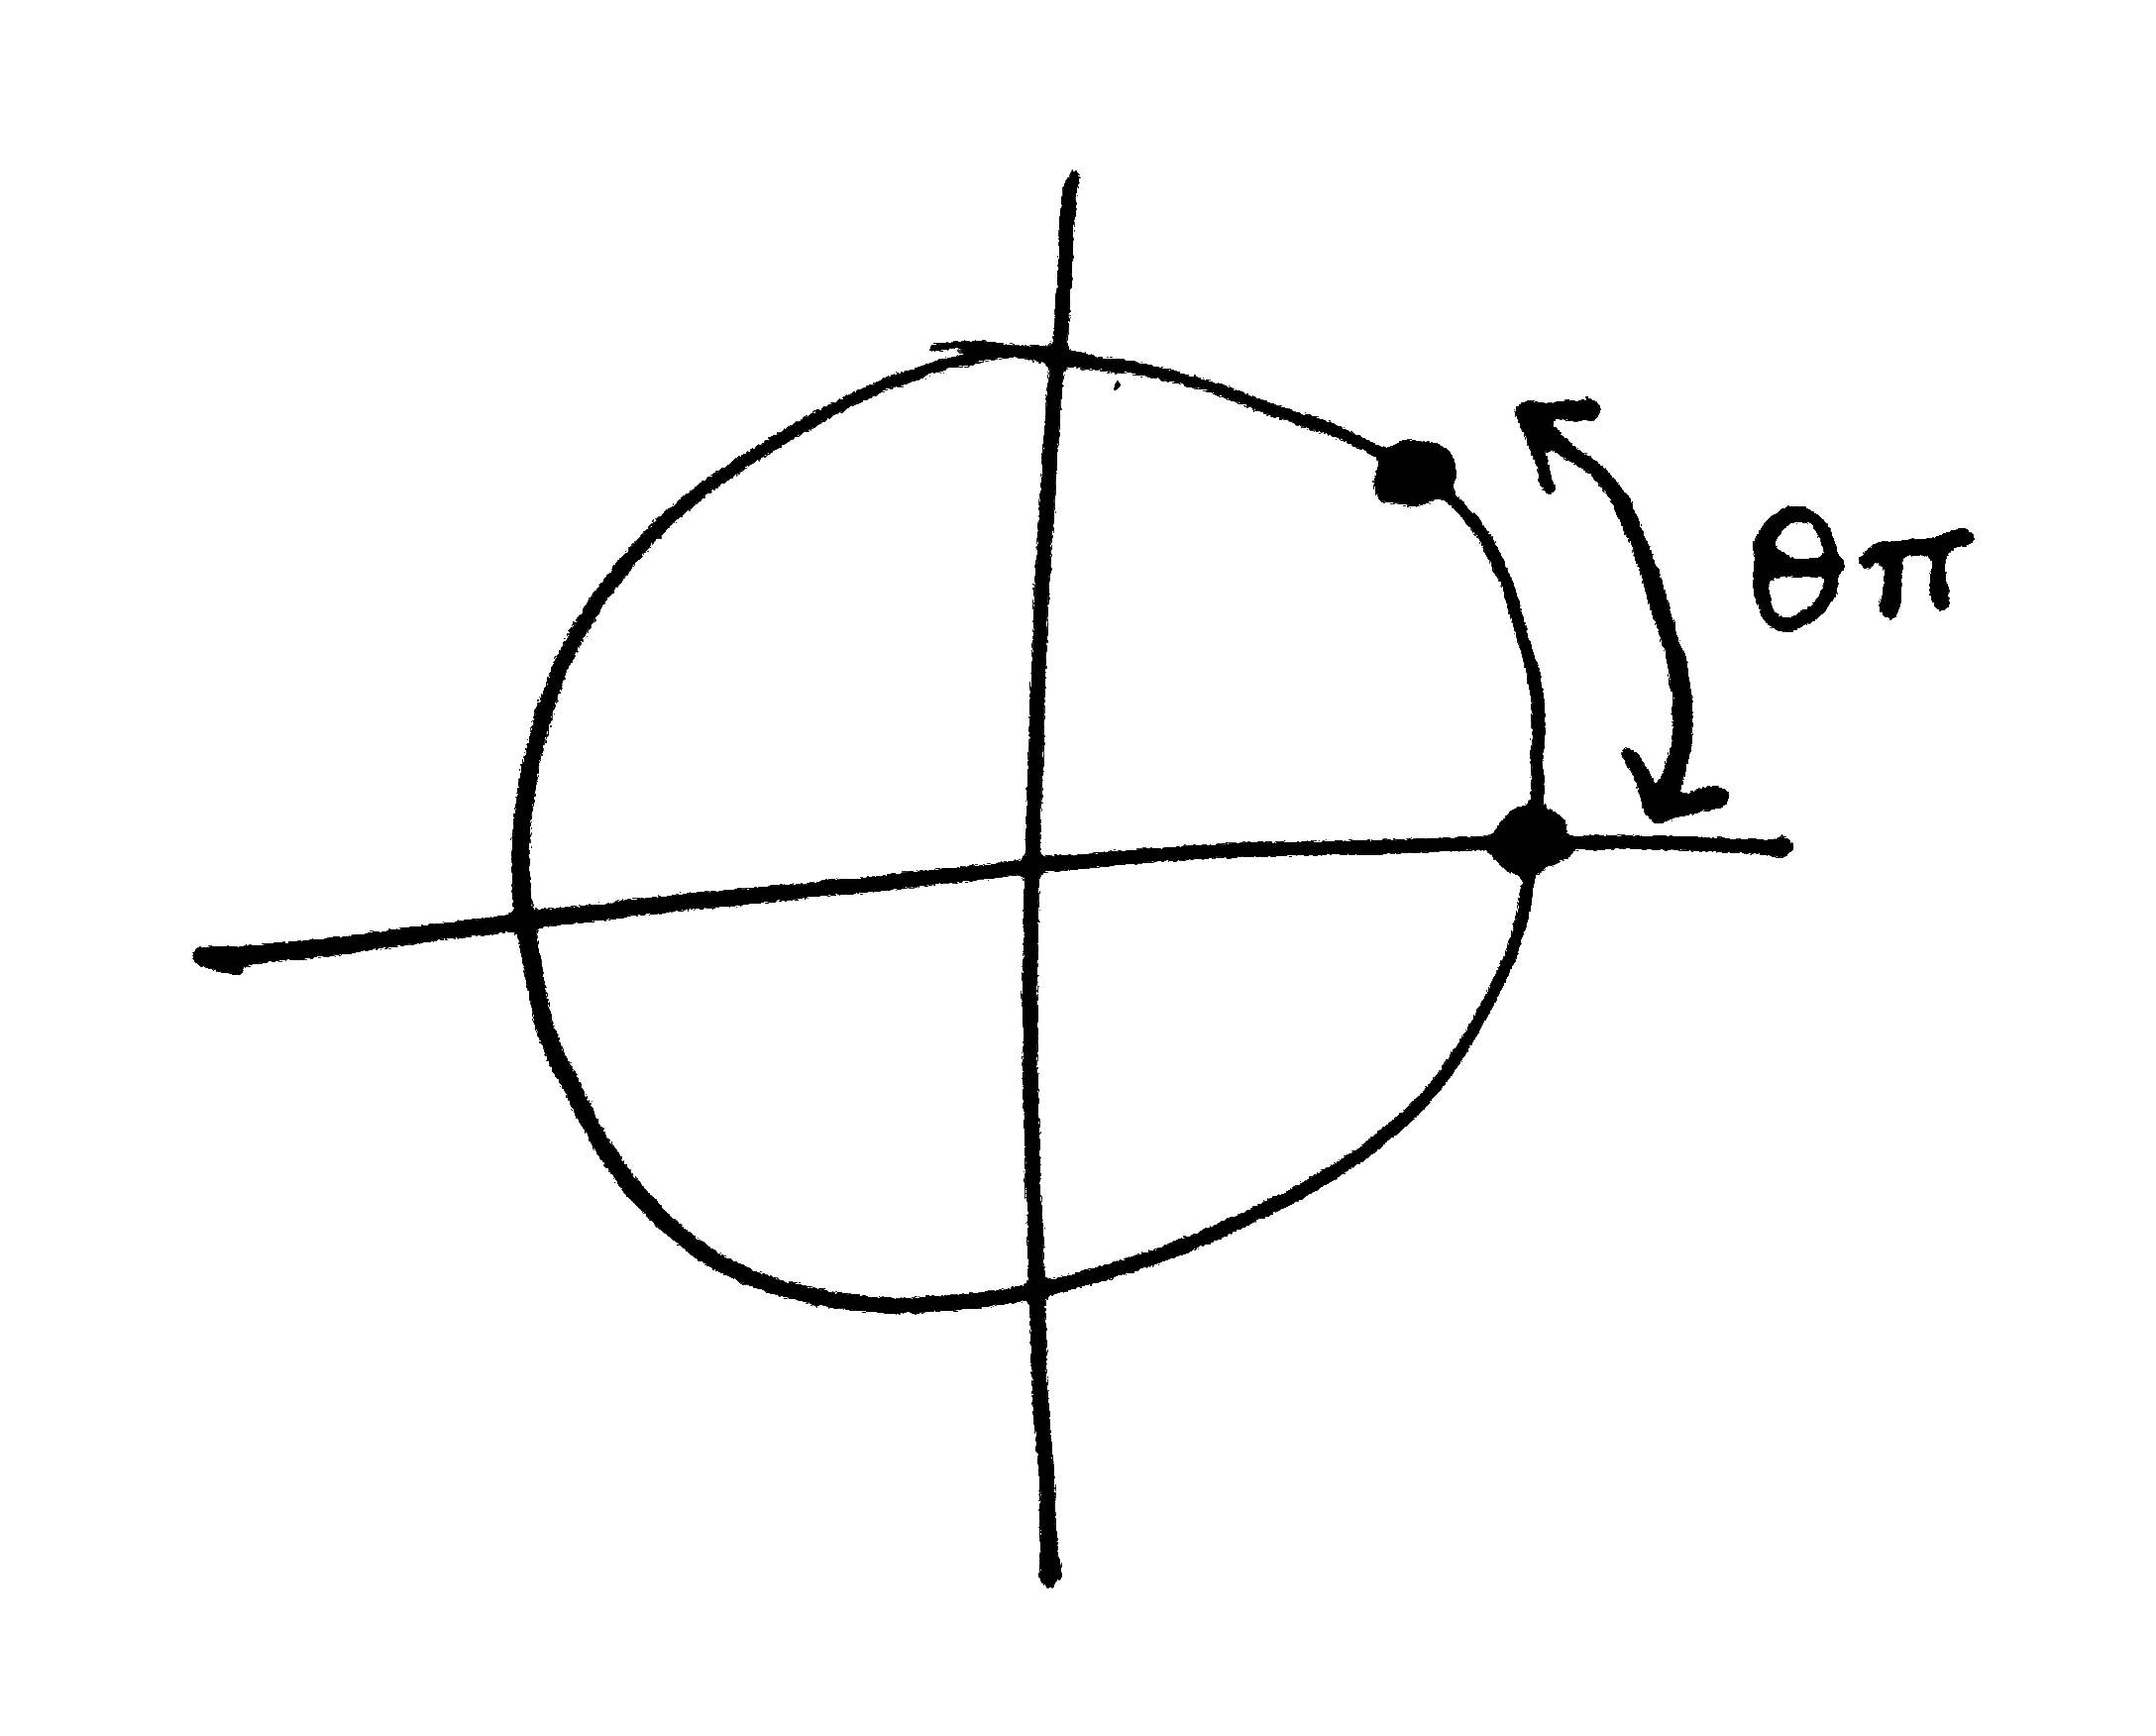
\includegraphics[width=0.5\linewidth]{img/abelian-phase-shift.jpg}
  \caption{The shift of energy levels due to an abelian phase $\theta$.}
  \label{fig: abelian phase shift}
\end{figure}
















\chapter{Physical realizability}

Conjectured that non-abelian states in FQH liquids at filling fraction $\nu = 5/2$ and $\nu = 12/5$. \cite{TODO} \cite{wang book}

``Braid Matrices and Quantum Gates for Ising Anyons Topological Quantum Computation'': \url{https://arxiv.org/abs/1003.1253}
``The most promising non-abelian anyon is the Ising $\sigma$ anyon in $\nu = 5/2$ FQH liquids.'' -- \cite[sec. 7.2]{wang book}


%%%%%%%%%%%%%%%%%%%%%%%%%%%%%%%%%%%%%%%%%%%%%%%%%%%%%%%%%%%%%%%%%%%%%%%%%%%%%%%%



\chapter{Topological Quantum Computation}

\section{Quantum computation}

The reader is assumed to be familiar with the basics of quantum computation. A good introduction to the subject can be found in \cite{nielsen chuang}.

Recall that time evolution of a quantum state $\ket{\psi}$ is unitary. If the quantum system is described by a Hamiltonian $H$, time evolution of $\ket{\psi}$ is governed by the Schrödinger equation $i\frac{\partial\ket{\psi}}{\partial t} = H\ket{\psi}$. For finite-dimensional state-spaces we get the solution $\ket{\psi_t} = e^{-itH}\ket{\psi_0}$. Since the Hamiltonian is hermitian, the time evolution operator $e^{-itH}$ is unitary.

%  Since H is Hermitian, e
% unitary matrix. Therefore we will just say states evolve by unitary matrices.
% In quantum computation, we apply unitary transformations to state
% vectors |ψ> to process the information encoded in |ψ>. Hence information
% processing in quantum computation is multiplication by unitary matrices



Explain notation in \cite{topological quantum compiling} via diagrams, i.e.

\begin{align*}
  (\bullet,\bullet)_0 &= \fs{\tau,\tau}{1,\tau,1} \\
  (\bullet,\bullet)_1 &= \fs{\tau,\tau}{1,\tau,\tau} \\
  ((\bullet, \bullet)_0 , (\bullet, \bullet)_0)_0 &= \fsfuseddouble{1}{\tau}{\tau}{1}{1}{\tau}{\tau}{1}{1} \\
  ((\bullet, \bullet)_1 , (\bullet, \bullet)_1)_0 &= \fsfuseddouble{1}{\tau}{\tau}{\tau}{\tau}{\tau}{\tau}{\tau}{\tau} \\
  ((\bullet, \bullet)_1 , \bullet)_0 &= \fs{\tau,\tau}{\tau,\tau,1} \\
  ((\bullet, \bullet)_0 , \bullet)_1 &= \fs{\tau,\tau}{\tau,1,\tau} \\
  ((\bullet, \bullet)_1 , \bullet)_1 &= \fs{\tau,\tau}{\tau,\tau,\tau}
\end{align*}



\section{??}


``One important problem is decoherence and systematic errors in unitary transformations which occur in real
quantum systems. From the purely theoretical point of view, this problem has been solved
due to Shor’s discovery of fault-tolerant quantum computation [2], with subsequent improvements
[3, 4, 5, 6]. An arbitrary quantum circuit can be simulated using imperfect gates, provided
these gates are close to the ideal ones up to a constant precision
$\delta$. Unfortunately, the threshold value of $\delta$ is rather small; it is very difficult to achieve this precision.'' \cite{kitaev fault-tolerant anyons} Started with \cite{shor fault-tolerant}, later improvements, discussed more in \cite{kitaev fault-tolerant anyons}.

``In the Abelian case the braiding results in phase factors that are both geometrical and dynamical in nature and thus hard to distinguish. On the contrary, the non-Abelian anyons cause a change in the amplitude of the participating states, which is easily distinguished from spurious dynamical phase factors.'' -- Preskill?

Solovay-Kitaev theorem:
``The Solovay-Kitaev (SK) theorem is one of the most important fundamental results in the
theory of quantum computation. In its simplest form the SK theorem shows that, roughly
speaking, if a set of single-qubit quantum gates generates a dense subset of SU(2), then that
set is guaranteed to fill SU(2) quickly, i.e., it is possible to obtain good approximations to
any desired gate using surprisingly short sequences of gates from the given generating set.'' -- \url{https://arxiv.org/pdf/quant-ph/0505030v2.pdf} see also \cite[Appendix 3]{nielsen chuang}


It is not known if there exists a braid that exactly represents the Pauli $x$-matrix up to a global phase. \cite[sec. 1.5]{wang book}

\begin{definition}{Quantum dimension $d_\alpha$}

  \cite{preskill}, and \cite[p. 388]{short intro fib}

  The number $d_\alpha(n)$ is the number of ways $n$ anyons of type $\alpha$ can be fused to yield an anyon of the same type $\alpha$. The quantum dimension $d_\alpha$ quantifies the rate of growth of the dimension $d_\alpha(n)$ of the Hilbert space of the fusion channels, in the sense that $d_\alpha(n) \to d_\alpha^n$ as $n\to\infty$. The quantum dimension satisfies the following product rule
  \begin{equation}\label{eq:quantum dimension product rule}
    d_a d_b = \sum_c N_{ab}^c.
  \end{equation}
  TODO Why?
  The number $d_\alpha$ is the unweighted probability that two $\alpha$ anyons fuse to an $\alpha$ anyon. TODO Why?
\end{definition}


``$S_{\text{topo}} = \log D$ where $D = \log \sqrt{\sum_j d_j^2}$ is the total quantum dimension.''









































\chapter{Quantum algorithms}

\begin{enumerate}
  \item \url{https://en.wikipedia.org/wiki/Deutsch%E2%80%93Jozsa_algorithm}
  \item Jan-Åke Larsson, Niklas Johansson - Efficient classical simulation of the Deutsch-Jozsa and Simon's algorithms, \url{http://arxiv.org/abs/1508.05027}
\end{enumerate}


\chapter{Category theory}

\url{http://research.microsoft.com/en-us/um/people/gurevich/opera/225.pdf} and reference 9 \url{http://www.cs.mcgill.ca/~prakash/Pubs/MTCanyons.pdf}

\begin{itemize}
  \item
    ``Category theory allows you to work on structures without the need first to pulverise them into set theoretic dust. To give an example from the field of architecture, when studying Notre Dame cathedral in Paris, you try to understand how the building relates to other cathedrals of the day, and then to earlier and later cathedrals, and other kinds of ecclesiastical building. What you don't do is begin by imagining it reduced to a pile of mineral fragments.'' -- Corfield, Towards a Philosophy of Real Mathematics p. 239.

  \item
    Any category with finite products give a monoidal category in which the unit object is the terminal object.

  \item
    TODO: Monoid in a category with finite products vs. monoid in a monoidal category?

  \item
    Fusion spaces as categories.

    Overview (good!) \url{http://www.cs.ox.ac.uk/bob.coecke/Eric.pdf}

    Appendix E in \url{https://arxiv.org/pdf/cond-mat/0506438v3.pdf} perhaps check this \url{https://arxiv.org/pdf/1307.8244v6.pdf} as well, and more general in the book Tensor Categories \url{http://www-math.mit.edu/~etingof/egnobookfinal.pdf}.

    \url{http://www.cs.mcgill.ca/~prakash/Pubs/MTCanyons.pdf}

    \url{http://mathoverflow.net/questions/243798/module-categories-for-fibonacci-anyons/243800}

    \url{http://physics.stackexchange.com/questions/27080/direct-sum-of-anyons}
\end{itemize}


\chapter{Möten}

\section{2016-02-01}

\subsection{Anteckningar}

Following the discussion of 2016-12-08.

\emph{Flyttade till chapter excl. principles etc}

\section{2016-12-08}

\subsection{Mail med sammanställning}

\begin{enumerate}
  \item Fundera på spektrumet för vinkeloperatorn med matris-randvillkor (t.ex. ta några konkreta exempel eller red ut för $U(2)$ med explicit parametrisering).
  \item Reda ut matrisen $U_p$ i ett konkret fall, t.ex. 2-6 anyoner i nån konkret icke-abelsk representation.
  \item Reda ut matrisen $U_p$ i allmännare fall, t.ex. alla N för Fibonacci eller Burau. Se om det finns nån speciell talteoretisk struktur som t.ex. udda heltal i den allmänna matrisens spektrum.
  \item Undersök konsekvenser för vinkeloperatorn, om dess spektrum är begränsat nedifrån för alla p. Förändras bilden mycket om man slänger på en extra abelsk fas?
\end{enumerate}

\subsection{Anteckningar}

\emph{Flyttade till chapter excl. principles etc}


\section{2016-11-17}

Eddy email:
\begin{quote}
  Jag bifogar en avhandling av Parsa Bonderson och ett papper
  som handlar om hur man beskriver `anyon teorier'. I pappret (kitaev06.pdf)
  handlar det om appendix E, som man kan läsa separat.

  Två papper som använder anyoner för att bygga gates med är:
  \begin{itemize}
    \item \url{https://arxiv.org/abs/quant-ph/0610111}
    \item \url{https://arxiv.org/abs/0903.2239}
  \end{itemize}

  Till sist ett papper som använder (lite, i alla fall) Burau representationer
  för att optimera qubitar:
  \begin{itemize}
    \item \url{https://arxiv.org/abs/1102.5029}
  \end{itemize}

  Till sist ett papper om exclusion statistik, i det abelska fallet:
  \begin{itemize}
    \item \url{https://arxiv.org/abs/cond-mat/9801272}
  \end{itemize}
\end{quote}




\section{2016-10-08}

\emph{Hans Hansson, Eddy Ardonne, Douglas Lundholm.}

\begin{itemize}
  \item Douglas gick visade hans modell av anyoner från fermioner/bosoner av två typer; hav/bad-partiklar och spår(trace)-partiklar. Speciellt den statistiska repulsionen.
  \item Diskussionen fortsatte mot icke-abelska anyoner, kan man göra samma typ av utbyte av två partiklar runt $p$ partiklar om de är icke-abelska? Tydligen fanns problem med detta, vilka?!
  \item Efter att fusionskanaler togs upp frågade jag hur sannolikheterna vid fusion hör ihop med kvantdimensionen, Eddy gav ett mycket bra svar där han även redogjorde för ``$F$-modellen''. Svaret på frågan var helt enkelt att $F$ matrisen beror på kvantdimensionen för anyonerna och $F$ bestämmer sannolikheten.
  \item Även abelska anyoner ryms i denna modell och ges av att $N_{ab}^c$ är nollskilld endast för ett $c$ (verkligen $c$? iaf att två anyoner endast kan fusioneras till en annan anyon).
  \item Efteråt pratade jag kort med douglas och vi tyckte att man skulle titta explicit på ett exempel för hur $F$-modellen ger abelska anyoner, och sedan göra enkel utväxling med 2 anyoner runt $p$ anyoner i det icke-abelska fallet, för ett konkret val av $F$-modell, kanske både Ising och Fibonacci.
\end{itemize}



\section{2016-10-04}

Circling around $p$ particles is described by
\begin{align*}
  U_p &= \sigma_1 \sigma_2 \cdots \sigma_p \sigma_{p+1} \sigma_p \cdots \sigma_2 \sigma_1
  U_0 &= \sigma_1 \\
  U_1 &= \sigma_1 \sigma_2 \sigma_1
\end{align*}
The corresponding Schrödinger equation is then
\begin{align*}
  \psi''(\theta) &= -\lambda \psi(\theta) \\
  \psi(1) &= U_p \psi(0)
\end{align*}
and the question is: How does $\lambda$ depend on $p$?.

\textbf{Similarity transformation between braid generators}
\begin{align*}
  \sigma_1 = A \sigma_2 A^*, \quad \quad
  \sigma_i \mapsto A \sigma_i A^*
\end{align*}

\textbf{Berry phase} The Berry phase is similar to the anyonic phase. The Berry phase is the the holonomy of the state space manifold $M$. See Nakahara -- Geometry, Topology and Physics, chap. 10.

\textbf{Magnetism is a curvature}

\textbf{Curvature in a hole} There is no curvature outside the hole, but when circling the hole one sees curvature. That is, the space is a cone around the hole.




\chapter{Confusion}

Frågor till Eddy

\begin{itemize}
  \item Why must one distinguish between an anyon and its type? Mentioned in ``A short introduction to anyon models'', page 385. In the categorical perspective, anyons are objects and types are isomorphism classes of objects.
  \item Interference experiments for higher-dimensional phases (i.e. unitary matrices)?
  \item Leakage, 3 fib. anyons with unconstrained total charge, or 4 anyons with total charge constrained to 1.
\end{itemize}

Find the smallest anyon model giving qutrits.

\section{Misc.}

The three Pauli matrices span $SU(2)$, so do the two generators of $B_3$. How does this work? The generators of $B_3$ are fewer than the Pauli matrices. Is the span of the braid generators only dense in $SU(2)$?

\section{Representation theory}

Same group, different representations $\implies$ different physics.

Preskill pages 15, 26, 28, 30, 31, \textbf{33}, \textbf{42}, 54

\begin{itemize}
  \item 33: Charge $\leftrightarrow$ irreducible repr.
  \item \textbf{31-32}: $G = S_3$, why $D \times D = A + C + F + G + H$?
  \item How is the group $G$ chosen, TODO: REF the minimal finite group for classical computation.
  \item \textbf{42}: Concrete example in SU(3) (octet representation etc.)
\end{itemize}

After discussion with Torbjörn:

\begin{itemize}
  \item Consider faithful representations.
  \item Look into some book on matrix groups (Kurtis).
  \item Problems in fusion rules, dimensions do not match up. Fusion looks like a tensor product that splits into direct sums. Cannot isolate particles (because of entanglement, perhaps particles can be seen as eigenvalues). It is not the particles that get a representation, it is the braiding that get a representation. Modular tensor categories is the appropriate structure for modeling fusion spaces.

  $1 \times 1 = 1$ indicates that the trivial particle has a one dimensional represenation (in a agreement with that it acts trivially and is abelian. However, $\tau \times \tau = 1 + \tau$ only matches up dimension-wise if $\tau$ has a one-dimensional representation, but it doesn't since it is non-Abelian.
\end{itemize}


Other:

\begin{itemize}
  \item Topological entropy: Dynamical systems: 3.4.
  \item Make reference to quark color in when comparing exotic quantum degrees of freedom TODO: REF
  \item Anyonic statistic vs spin: Anyonic spin-statistic theorem?
  \item Fusion: Betyder $a\otimes b = c \oplus d$ att både $c$ och $d$ genereras, eller att $c$ eller $d$ genereras? Borde vara att båda genereras eftersom $N_{ab}^c \in \mathbb{Z}$, annars skulle vi kunna har $N_{ab}^c \in \mathbb{R}$ och tolka dem som sannolikheter?
  \item Sida 7 i ``Why should anyone care about computing with anyons?'' Fibonacci anyon realisering av qbuit.
  \item How to create anyons from the vacuum (total charge 0) vs. anyons with full total charge?
  \item Fibonacci model is the simplest non-Abelian model that is capable of universal quantum computation. Argument for why Abelian anyons do not suffice.
  \item What if the underlying 2D space is not Euclidean, perhaps a torus, or any 2D manifold?
\end{itemize}




\begin{thebibliography}{99}
  \bibitem{nakahara} Nakahara: Geometry, Topology and Physics. En trevlig och koncis introduktion till homotopi-grupper finns i kap 4, kap 2-3 kan dock behövas som förkunskaper. Denna bok har tidigare funnits på kårbokhandeln och tycker jag är helt klart värd att investera i, annars kolla biblioteket eller kontakta mig. Observera att man kan hoppa över kap 1 för matematiken.
  \bibitem{nayak} Nayak et al: En review om icke-abelska anyoner och kvantdatorer. Se section II.A.1
  \bibitem{artin} Artin: En av de mest fundamentala artiklarna om braidgruppen. Obs: svår! förväntas inte läsas, detsamma gäller för tillfället följande:
  \bibitem{mancarella} Mancarella et al: \verb|http://dx.doi.org/10.1016/j.nuclphysb.2012.10.020|
  \bibitem{birman-brendle} Birman, Brendle: \verb|http://www.math.columbia.edu/~jb/Handbook-21.pdf|, kapitel 4
  \bibitem{lundholm-solovej} Lundholm, Solovej: \verb|http://dx.doi.org/10.1007/s00220-013-1748-4|, Matematisk bakgrund samt exklusionsprincip för abelska anyoner.

  \bibitem{nielsen chuang}
    M. Nielsen, I. Chuang.
    \textit{Quantum computation and quantum information.}
    Cambridge university press (2010).

  \bibitem{preskill}
    J. Preskill.
    \textit{Lecture Notes for Physics 219: Quantum Computation, Chapter 9: Topological quantum computation}.
    \\
    \url{http://www.theory.caltech.edu/~preskill/ph219/topological.pdf}

  \bibitem{short intro fib}
    S. Trebst, M. Troyer, Z. Wang and A. W. W. Ludwig.
    \textit{A Short Introduction to Fibonacci Anyon Models.}
    Progress of Theoretical Physics Supplement No. 176, 2008.
    \\
    \url{http://stationq.cnsi.ucsb.edu/~wang/Publications/34.pdf}

  \bibitem{kitaev}
    A. Kitaev.
    \textit{Anyons in an exactly solved model and beyond.}
    Annals of Physics 321 (2006) 2.
    (Revised version \href{https://arxiv.org/abs/cond-mat/0506438}{arXiv:cond-mat/0506438}.)
    \\\relax
    [One of the founding papers. See especially Appendix E.]

  \bibitem{freedman kitaev larsen wang}
    M. Freedman, A. Kitaev, M. Larsen and Z. Wang.
    \textit{Topological quantum computation.}
    American mathematical society, vol 40, p. 31–38.
    \\
    \url{http://dx.doi.org/10.1090/S0273-0979-02-00964-3}

  \bibitem{shor fault-tolerant}
    P. Shor.
    \textit{Fault-tolerant quantum computation.}
    \href{https://arxiv.org/abs/quant-ph/9605011}{arXiv:quant-ph/9605011}

  \bibitem{kitaev fault-tolerant anyons}
    A. Kitaev.
    \textit{Fault-tolerant quantum computation by anyons.}
    \\
    \href{https://arxiv.org/abs/quant-ph/9707021}{arXiv:quant-ph/9707021}

  \bibitem{topological quantum compiling}
    L. Hormozi, G. Zikos, N. Bonesteel, S. Simon.
    \textit{Topological quantum compiling.}
    Phys. Rev. B 75, 165310 (2007), \href{https://arxiv.org/abs/quant-ph/0610111}{arXiv:quant-ph/0610111}
    \\
    \url{http://link.aps.org/doi/10.1103/PhysRevB.75.165310}

  % The is the prequel to the above
  \bibitem{}
    N. Bonesteel, L. Hormozi, G. Zikos, and S. Simon.
    \textit{Braid topologies for quantum computation.}
    Phys. Rev. Lett. 95 (2005), 140503.

  \bibitem{asymptotical top compl}
    V. Kliuchnikov, A. Bocharov, K. Svore.
    \textit{Asymptotically optimal topological quantum compiling.}
    \\
    \href{https://arxiv.org/abs/1310.4150}{arXiv:1310.4150}

  \bibitem{pachos book}
    J. Pachos.
    \textit{Introduction to Topological Quantum Computation.}
    Cambridge University Press.
    \\
    \url{http://quantum.leeds.ac.uk/jiannis-pachos/book.html}
    \\
    \url{http://quantum.leeds.ac.uk/fileadmin/user_upload/Jiannis/IntroTQC.pdf}

  \bibitem{wang book}
    Z. Wang.
    \textit{Topological Quantum Computation.}
    Microsoft Research Station Q, University of California.
    AMS and CBMS.
    \url{http://www.math.ucsb.edu/~zhenghwa/data/course/cbms.pdf}

  \vspace{1cm}
  \hrule
  Possible references, perhaps not needed
  \hrule

  \bibitem{}
    M. Freedman, M. Larsen, Z. Wang.
    \textit{A modular functor which is universal for quantum computation.}
    \\
    \url{https://arxiv.org/pdf/quant-ph/0001108v2.pdf}


  \bibitem{oskar}
    O. Weinberger.
    \textit{Bachelor's thesis: The braid group, representations and non-abelian anyons}

  \bibitem{configuration spaces}
    E. Fadell, L. Neuwirth.
    \textit{Configuration spaces.}
    Math. Scand. 10 (1962) 111–118

  \bibitem{feynmann path integral}
    R. P. Feynman.
    \textit{Space-time approach to non-relativistic quantum mechanics.}
    Rev. Mod. Phys. 20 (1948) 367–387.

  \bibitem{feynmann path integrals indistinguishable particles}
    M. G. G. Laidlaw, C. M. DeWitt.
    \textit{Feynman functional integrals for systems of indistinguishable particles.}
    Phys. Rev. D 3 (1971) 1375–1378.

  \bibitem{fröhlich}
    J. Fröhlich.
    \textit{Quantum statistics and locality.}
    Proceedings of the gibbs symposium,
    Yale University, May 15-17, 1989

  \bibitem{bonderson}
    P. H. Bonderson
    \textit{Non-Abelian Anyons and Interferometry.}
    (2007) Ph.D Thesis

  \bibitem{mac lane}
    S. Mac Lane, Categories for the Working Mathematician, 2nd Edition, Graduate Texts in Mathematics, Springer-Verlag, New York, 1998.

\end{thebibliography}

\end{document}
